\begin{figure}
    \centering
    \begin{tabular}{cc}
        \subfloat[][$B^0 \to D(K\pi)K^{*0}$ Run 1]{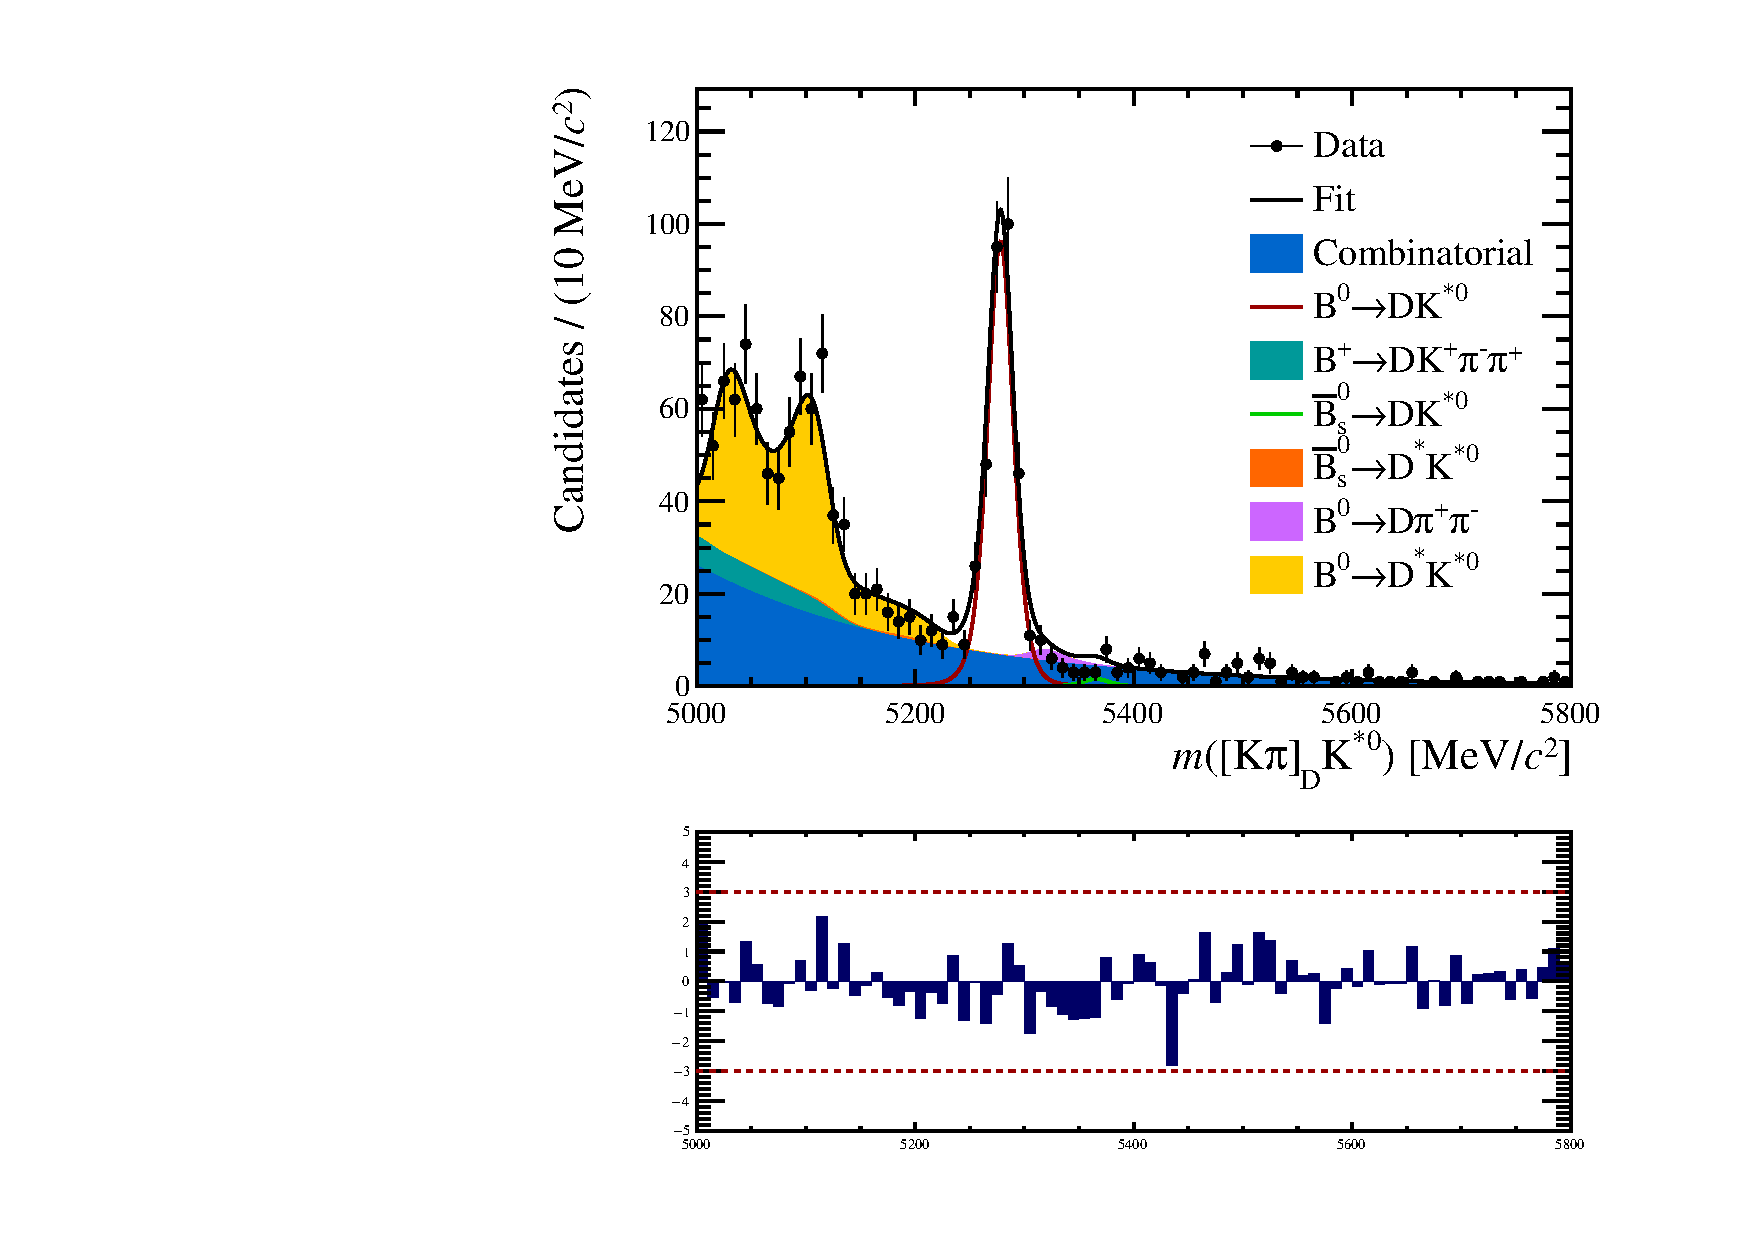
\includegraphics[width=0.45\textwidth]{ANA_resources/Plots/Data_fit/twoAndFourBody_data_split_Kpi_run1_plus.pdf}} &
        \subfloat[][$\bar{B}^0 \to D(K\pi)\bar{K}^{*0}$ Run 1]{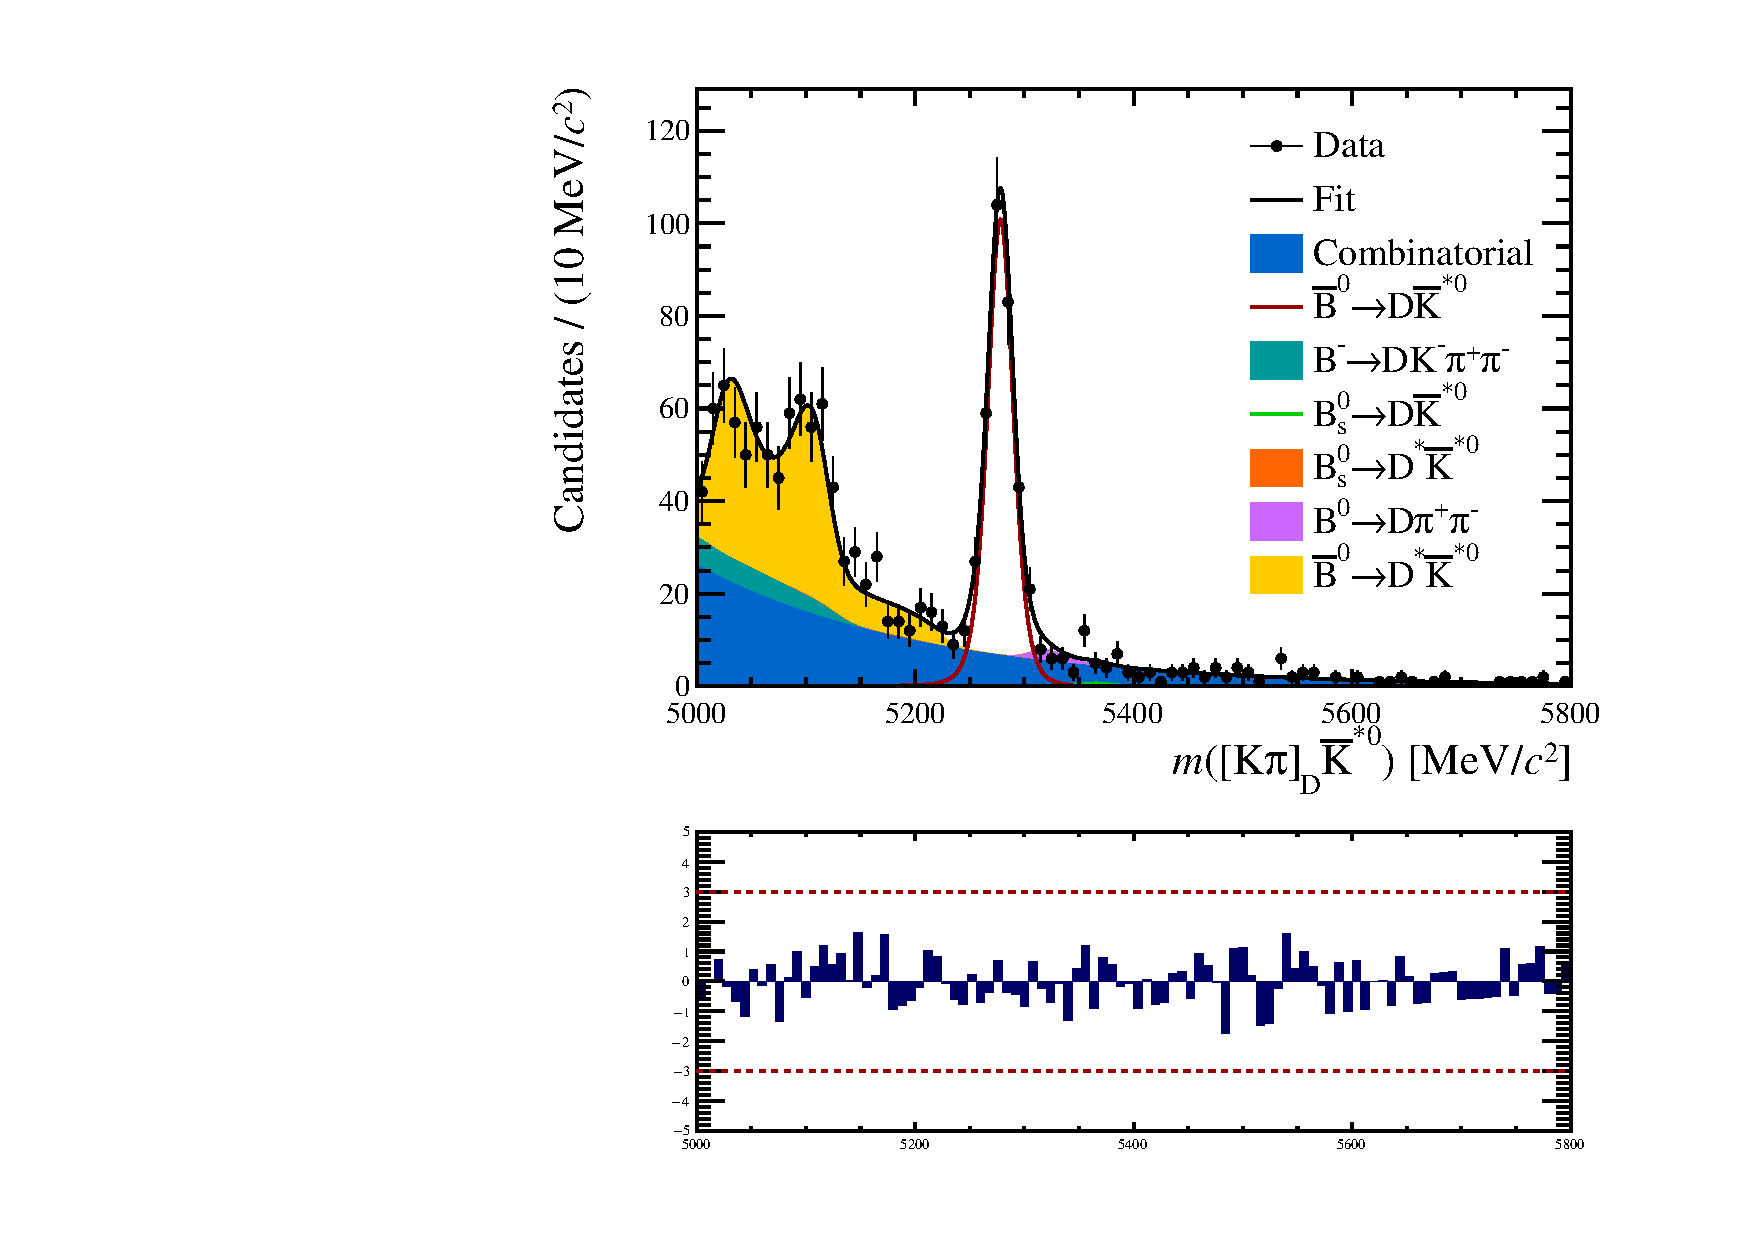
\includegraphics[width=0.45\textwidth]{ANA_resources/Plots/Data_fit/twoAndFourBody_data_split_Kpi_run1_minus.pdf}} \\
        \subfloat[][$B^0 \to D(K\pi)K^{*0}$ Run 2]{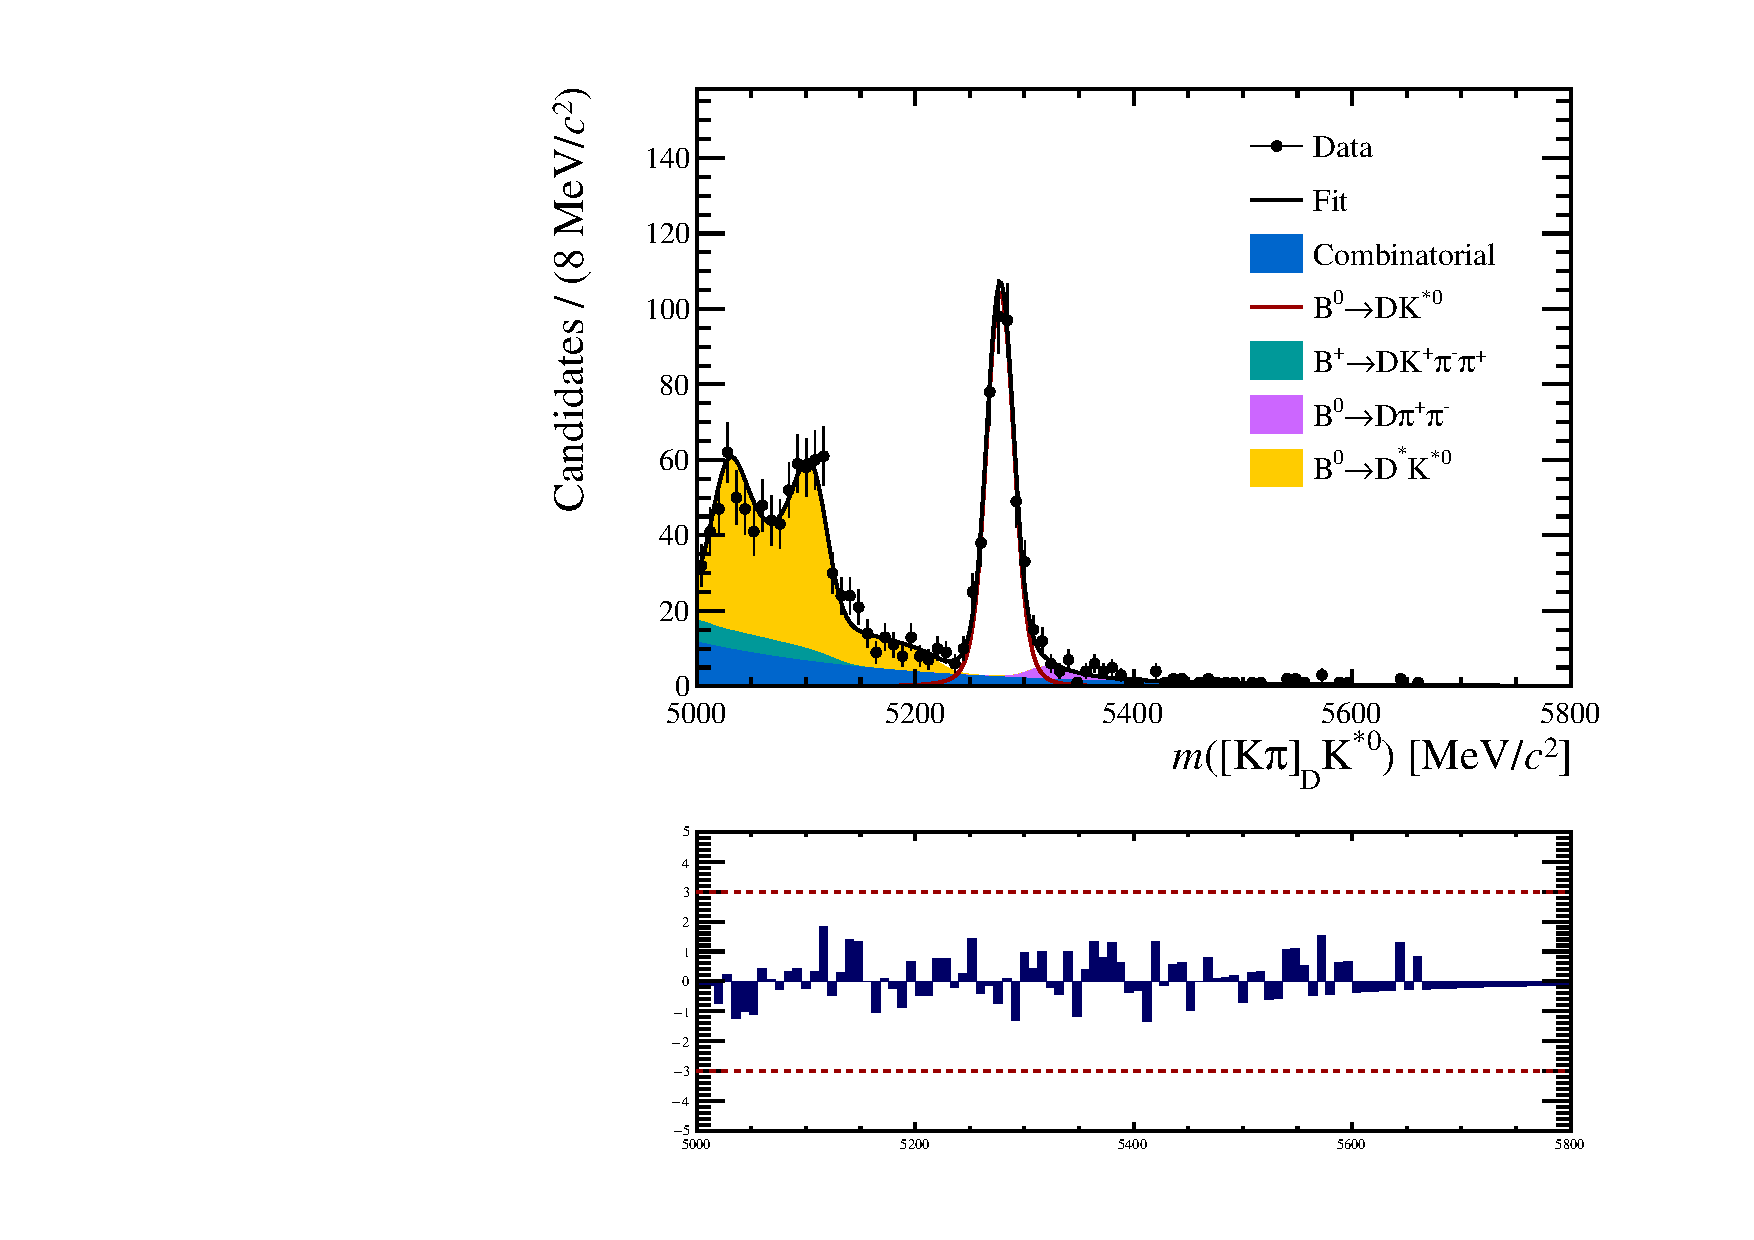
\includegraphics[width=0.45\textwidth]{ANA_resources/Plots/Data_fit/twoAndFourBody_data_split_Kpi_run2_plus.pdf}} &
        \subfloat[][$\bar{B}^0 \to D(K\pi)\bar{K}^{*0}$ Run 2]{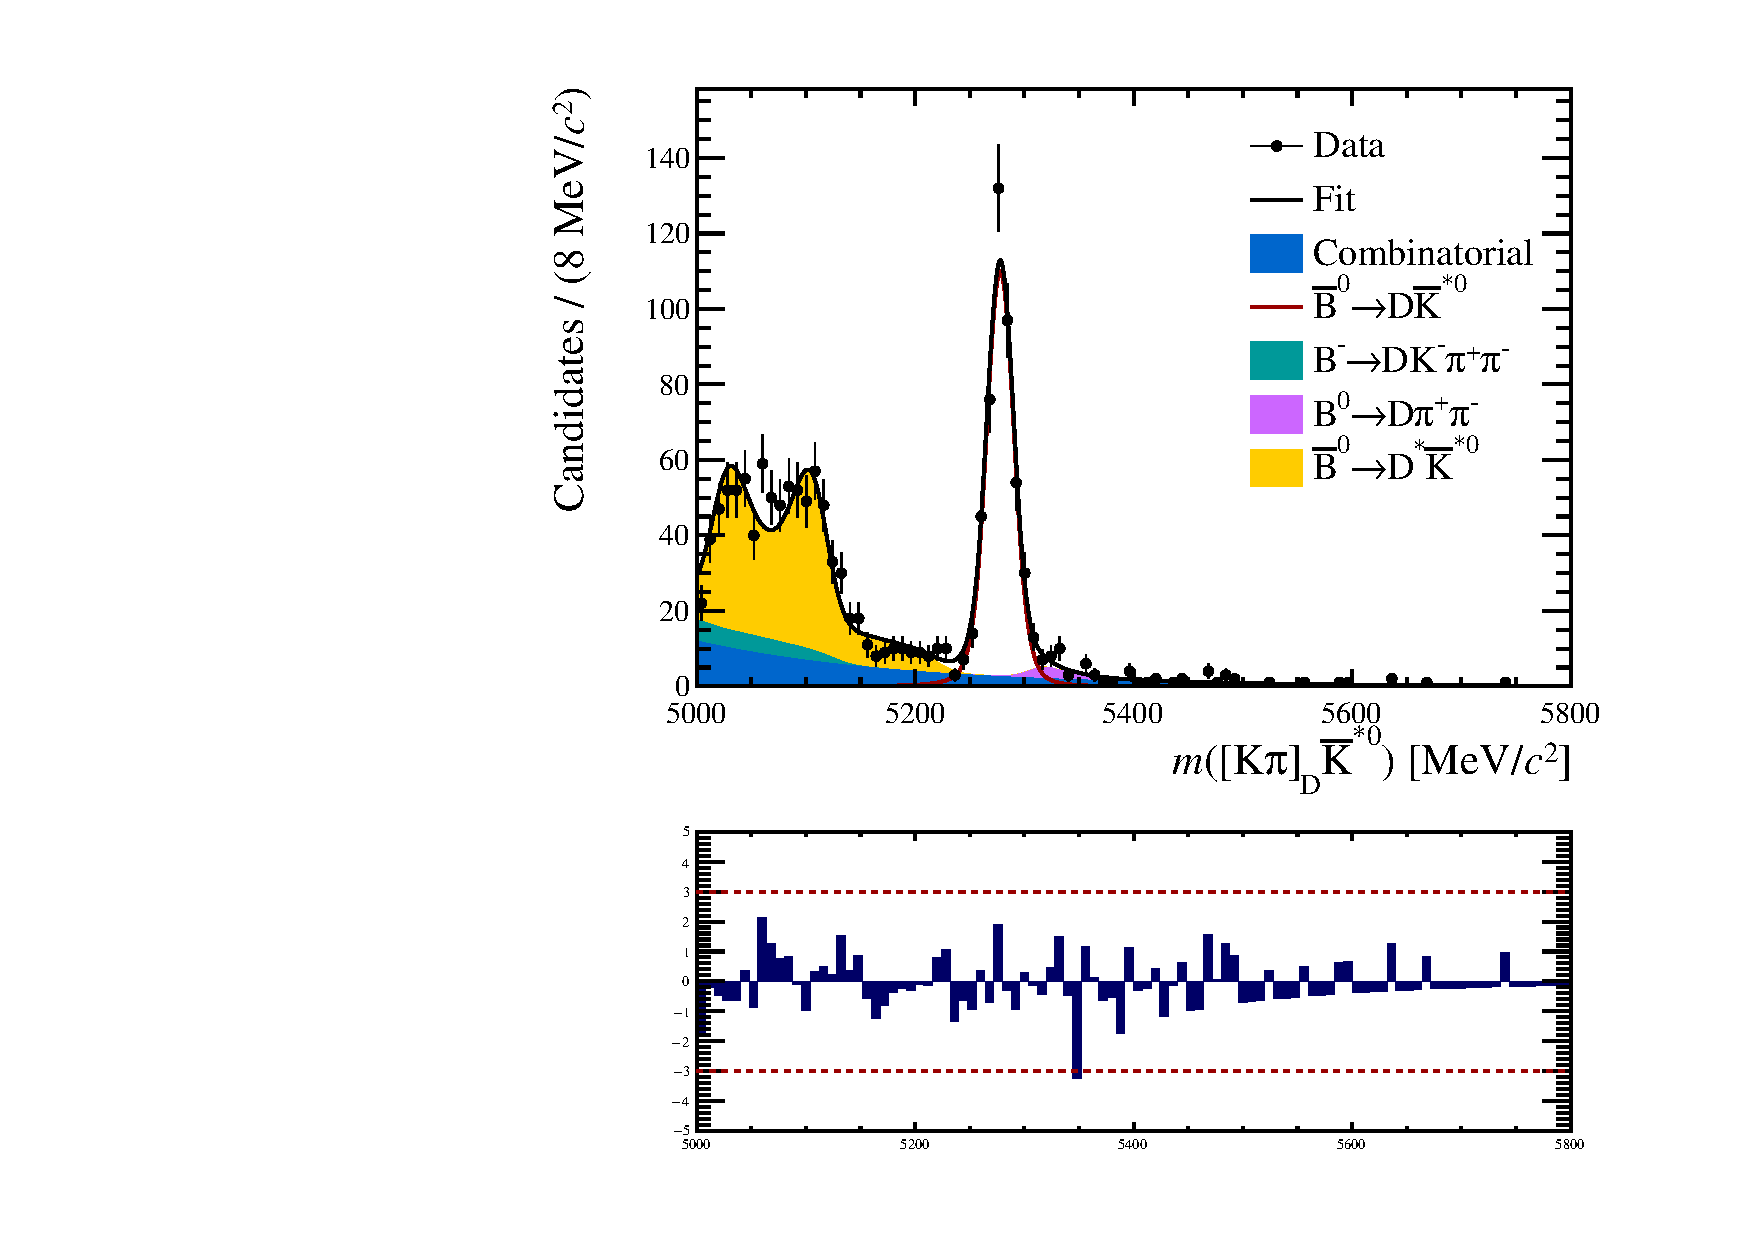
\includegraphics[width=0.45\textwidth]{ANA_resources/Plots/Data_fit/twoAndFourBody_data_split_Kpi_run2_minus.pdf}} \\
    \end{tabular}
    \caption{Fit to $B$ invariant mass of selected candidates in the $K\pi$ final state, split by $B$ flavour and run.}
\label{fig:data_fit_Kpi}
\end{figure}
\begin{figure}
    \centering
    \begin{tabular}{cc}
        \subfloat[][$B^0 \to D(\pi K)K^{*0}$ Run 1]{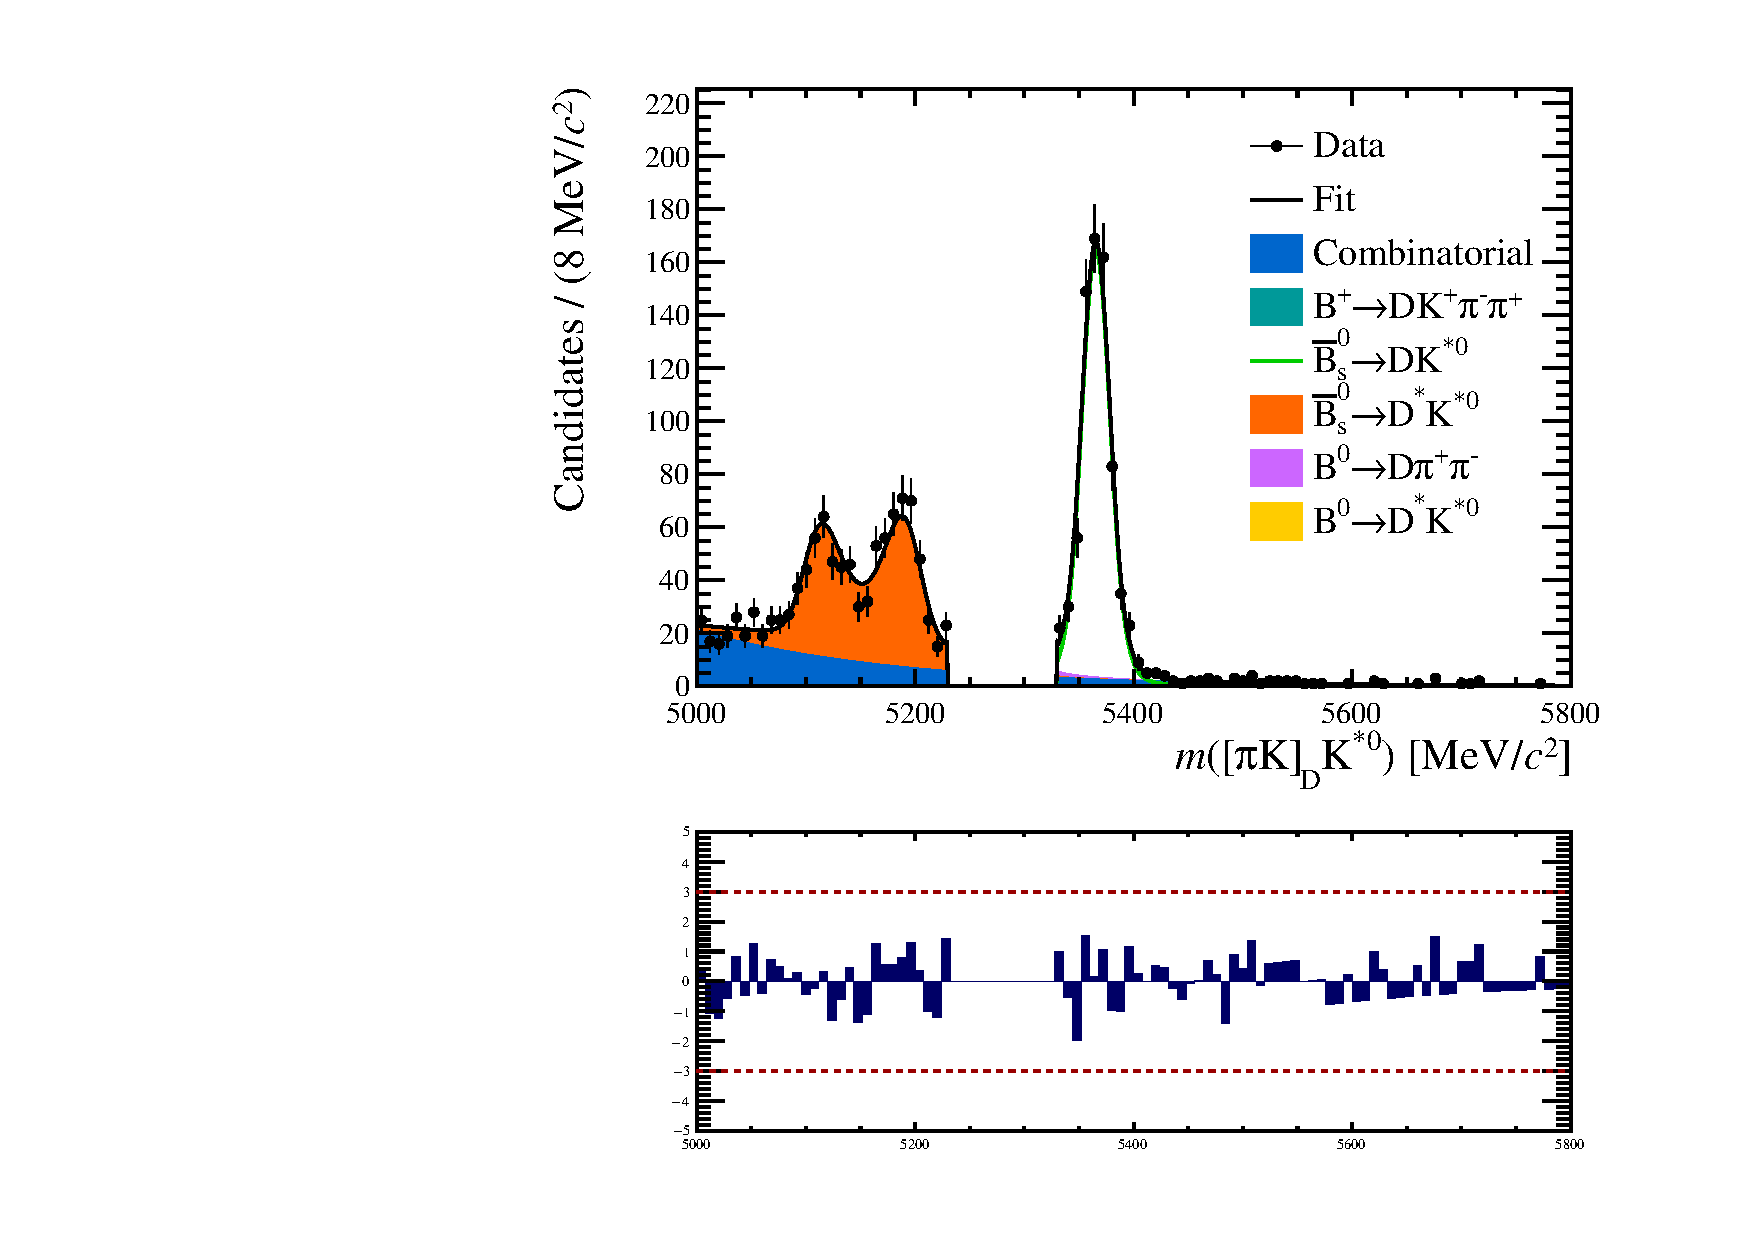
\includegraphics[width=0.45\textwidth]{ANA_resources/Plots/Data_fit/twoAndFourBody_data_split_piK_run1_plus.pdf}} &
        \subfloat[][$\bar{B}^0 \to D(\pi K)\bar{K}^{*0}$ Run 1]{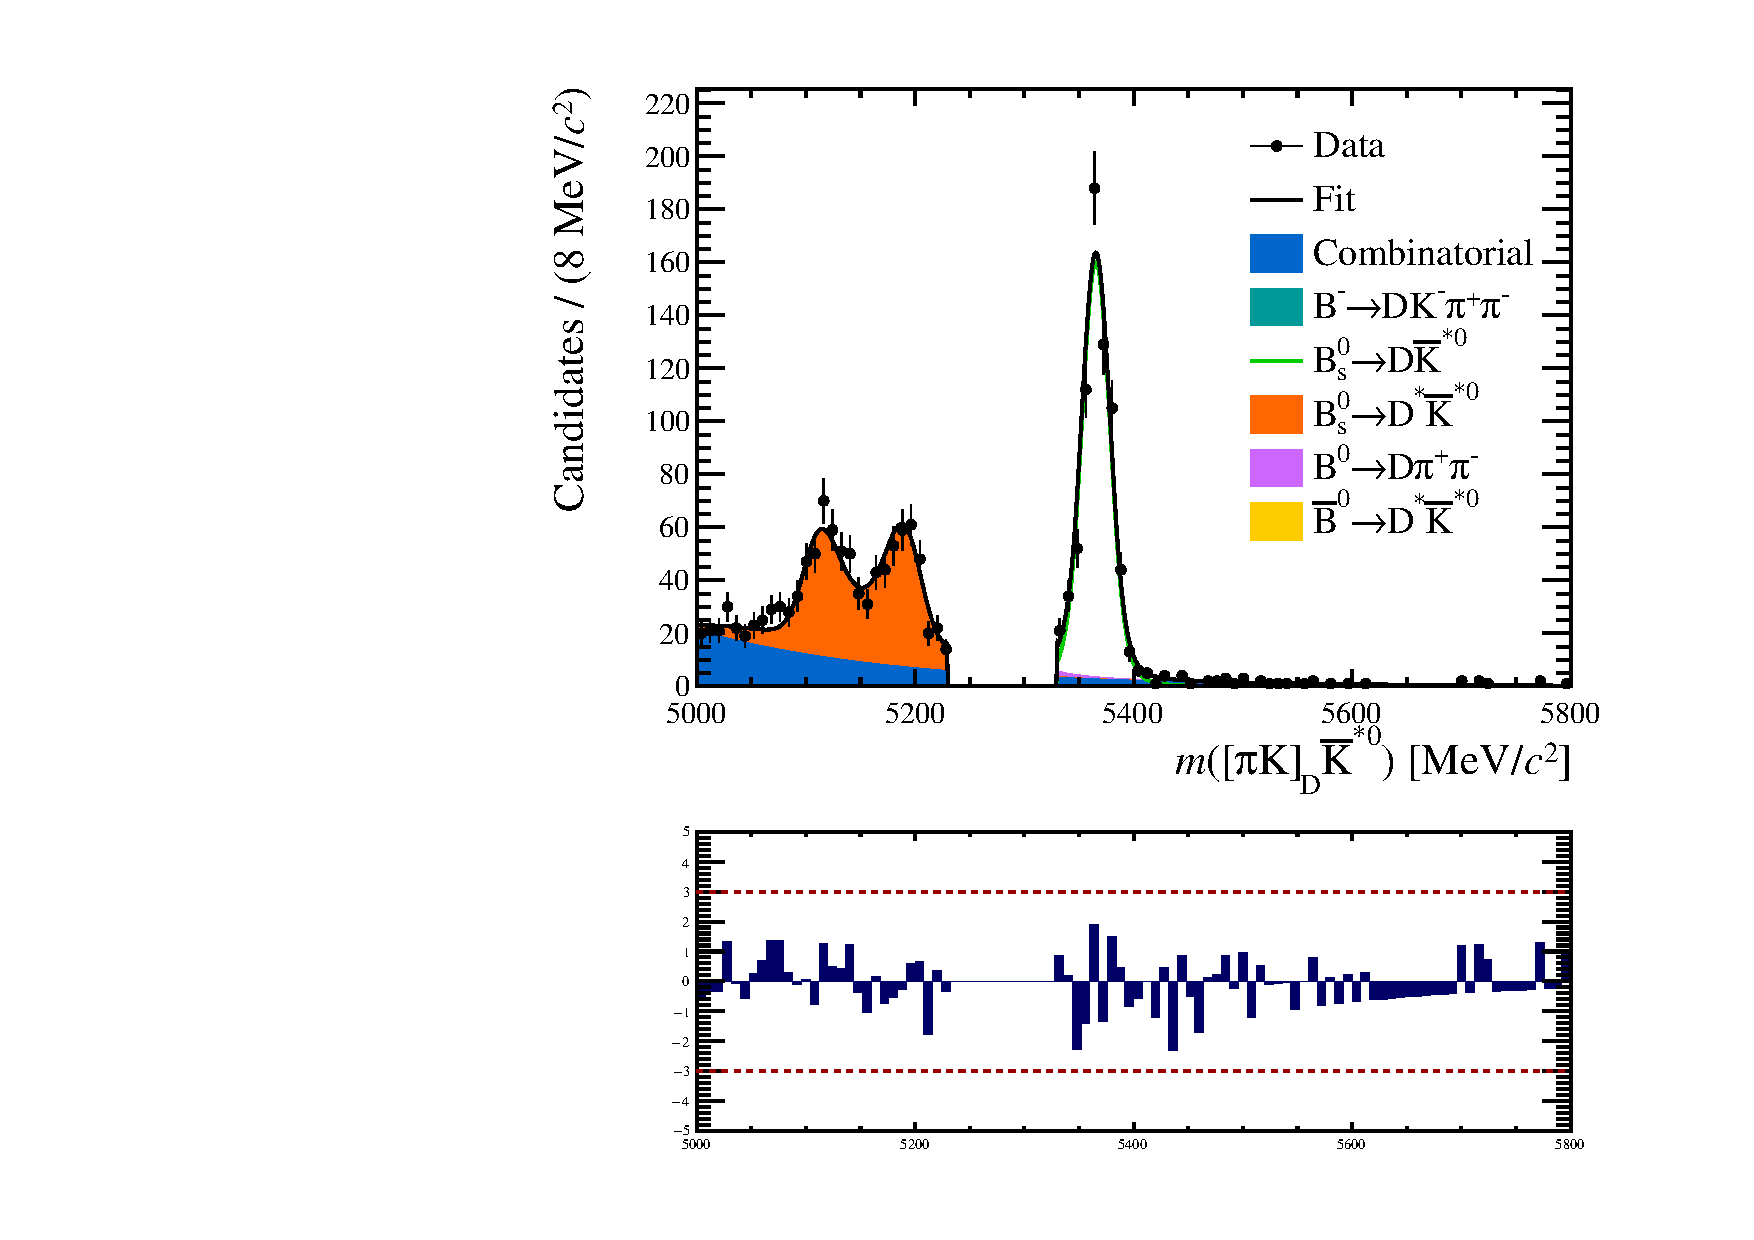
\includegraphics[width=0.45\textwidth]{ANA_resources/Plots/Data_fit/twoAndFourBody_data_split_piK_run1_minus.pdf}} \\
        \subfloat[][$B^0 \to D(\pi K)K^{*0}$ Run 2]{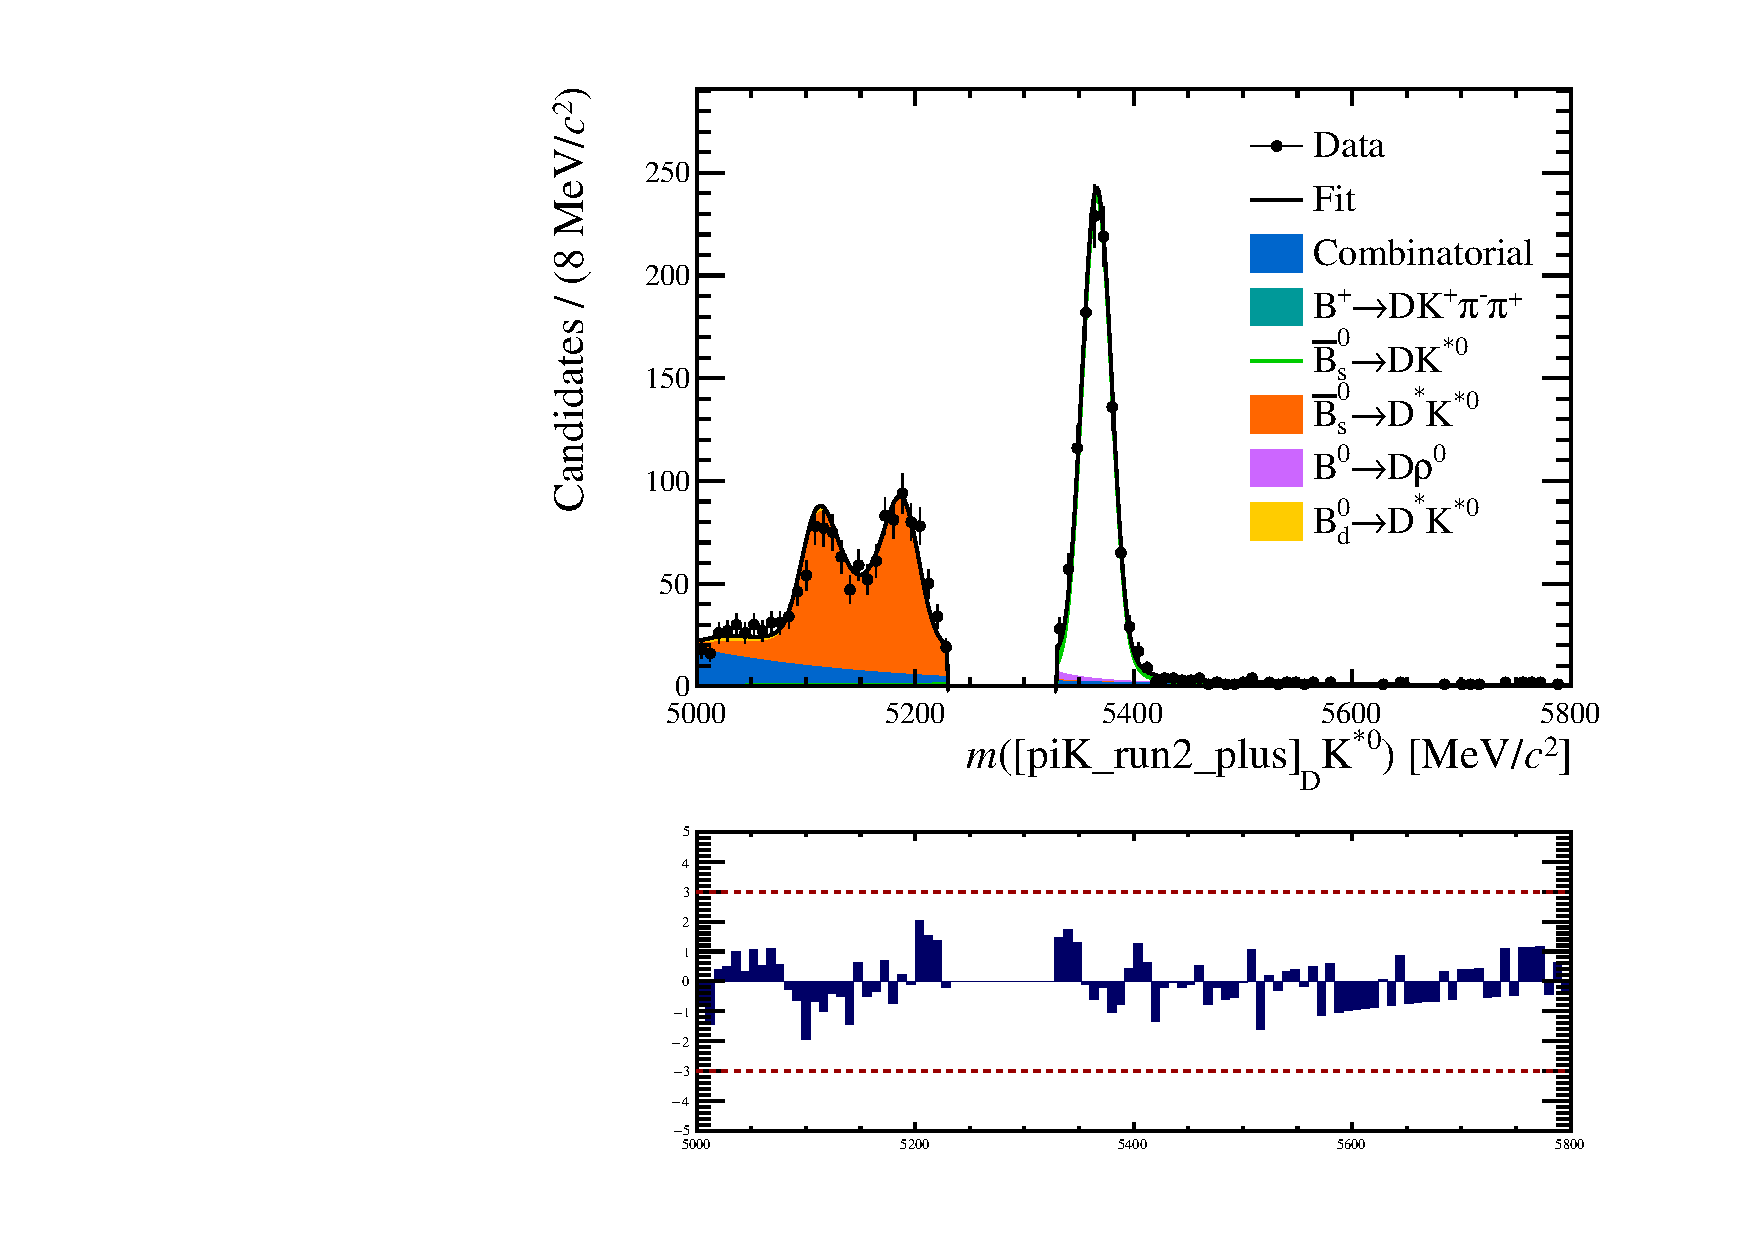
\includegraphics[width=0.45\textwidth]{ANA_resources/Plots/Data_fit/twoAndFourBody_data_split_piK_run2_plus.pdf}} &
        \subfloat[][$\bar{B}^0 \to D(\pi K)\bar{K}^{*0}$ Run 2]{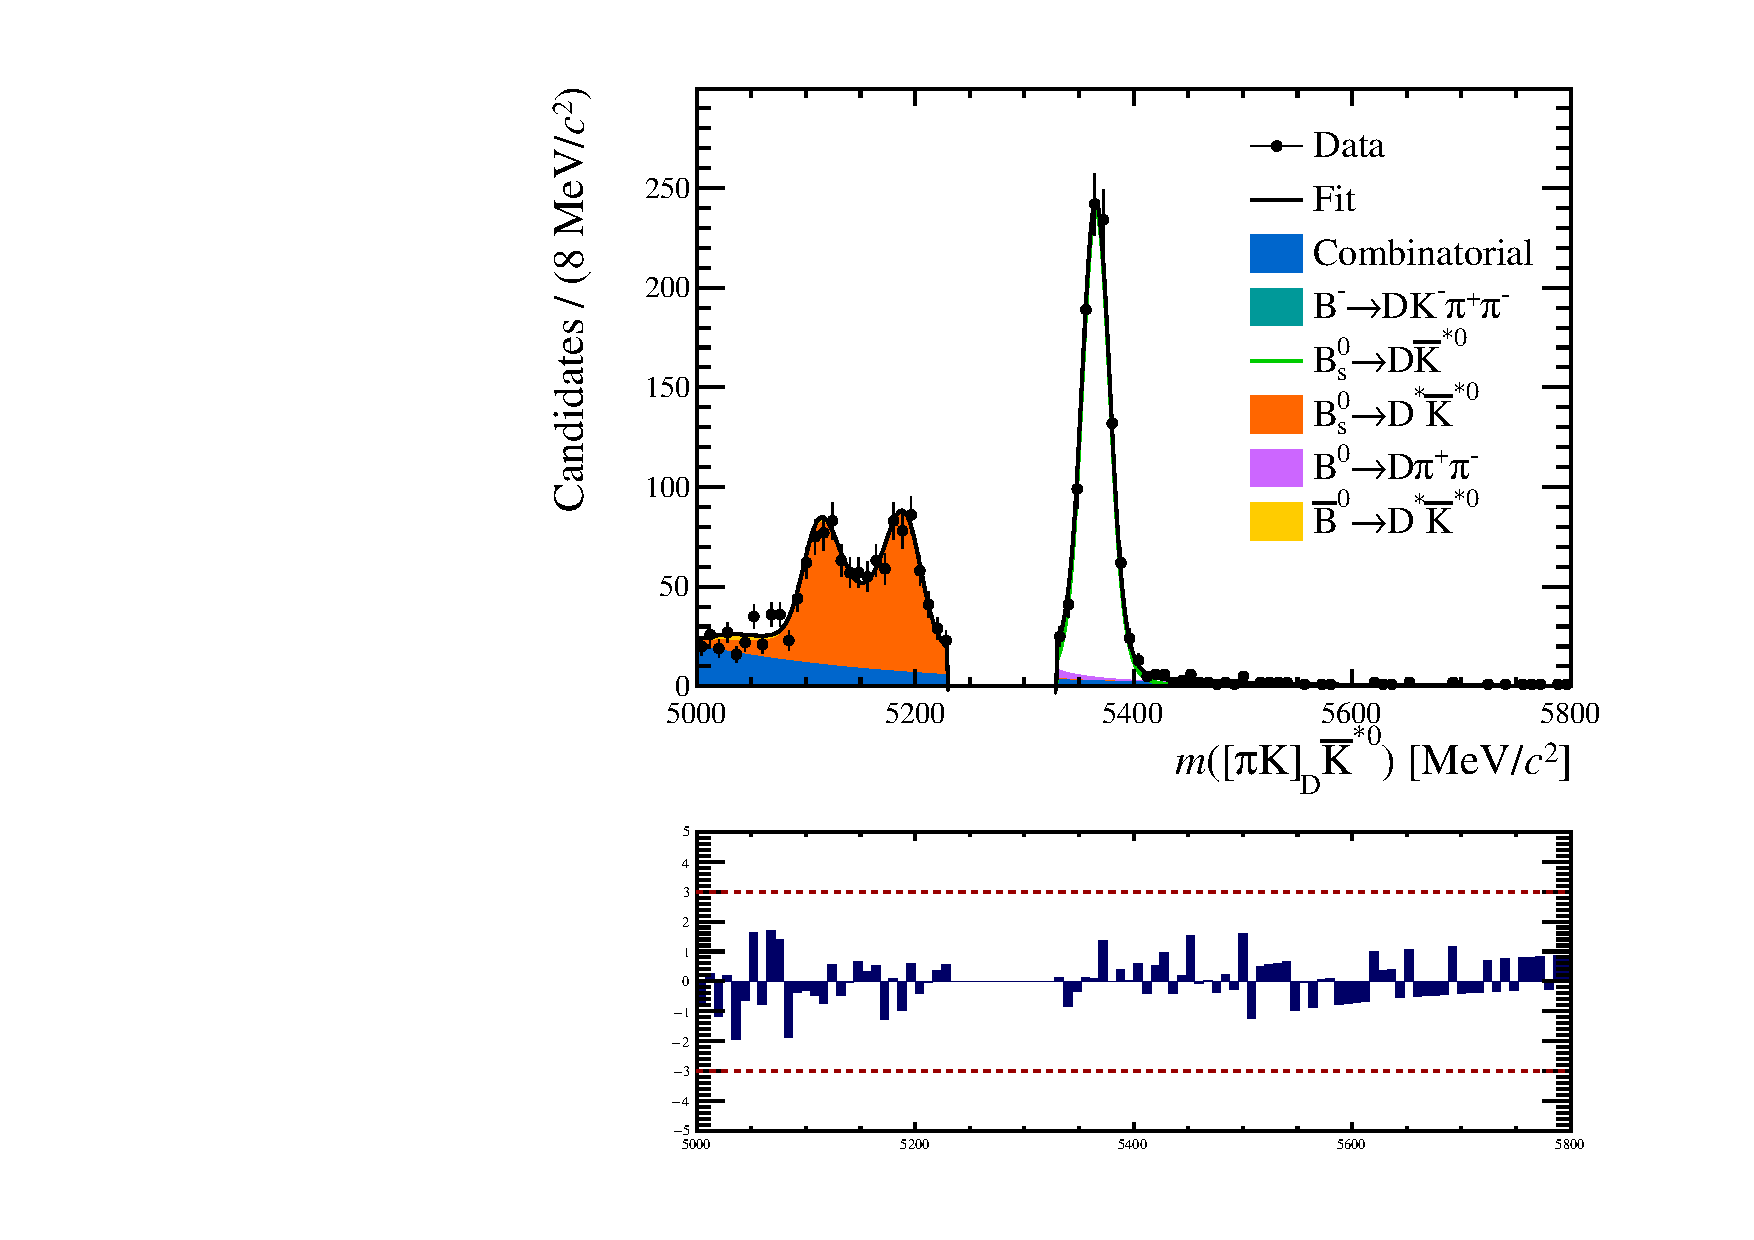
\includegraphics[width=0.45\textwidth]{ANA_resources/Plots/Data_fit/twoAndFourBody_data_split_piK_run2_minus.pdf}} \\
    \end{tabular}
    \caption{Fit to $B$ invariant mass of selected candidates in the $\pi K$ final state, split by $B$ flavour and run.}
\label{fig:data_fit_piK}
\end{figure}
\begin{figure}
    \centering
    \begin{tabular}{cc}
        \subfloat[][$B^0 \to D(KK)K^{*0}$ Run 1]{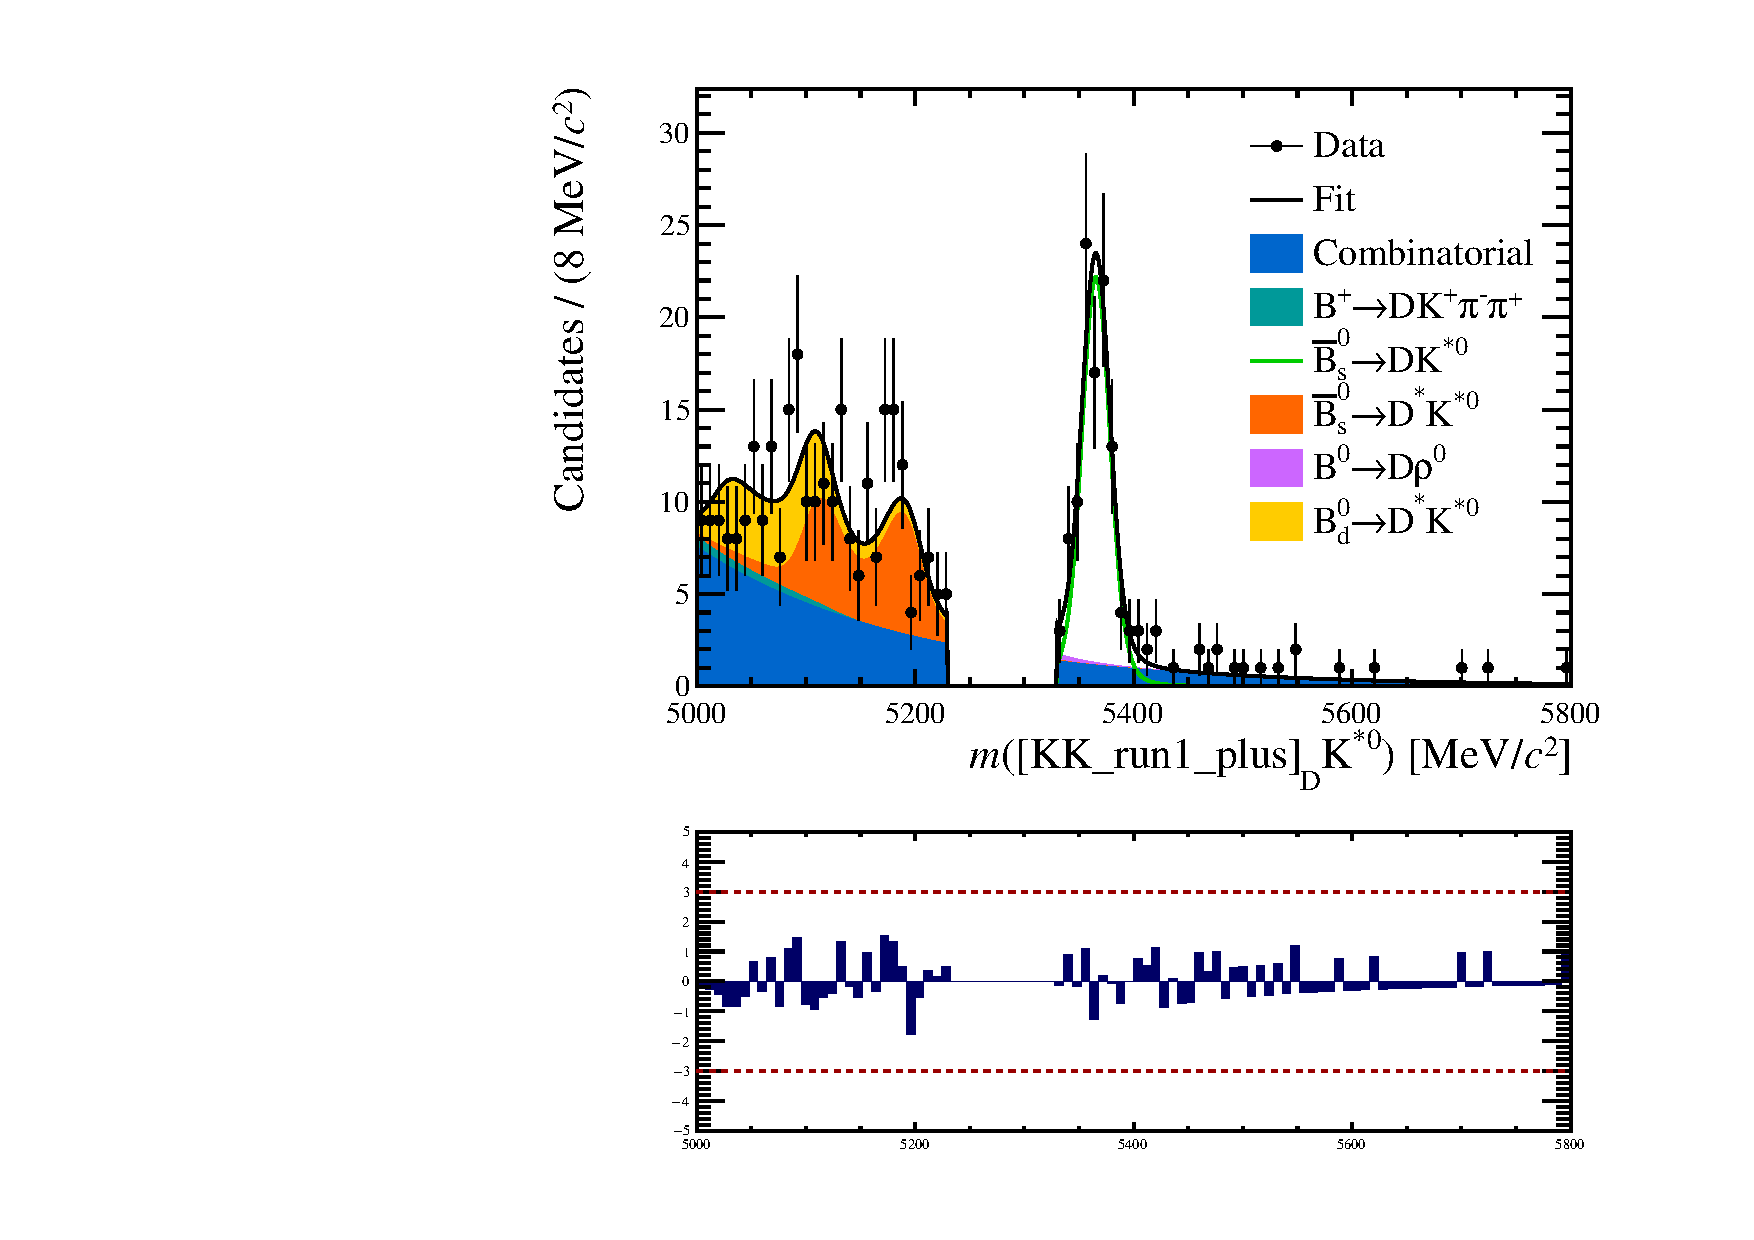
\includegraphics[width=0.45\textwidth]{ANA_resources/Plots/Data_fit/twoAndFourBody_data_split_KK_run1_plus.pdf}} &
        \subfloat[][$\bar{B}^0 \to D(KK)\bar{K}^{*0}$ Run 1]{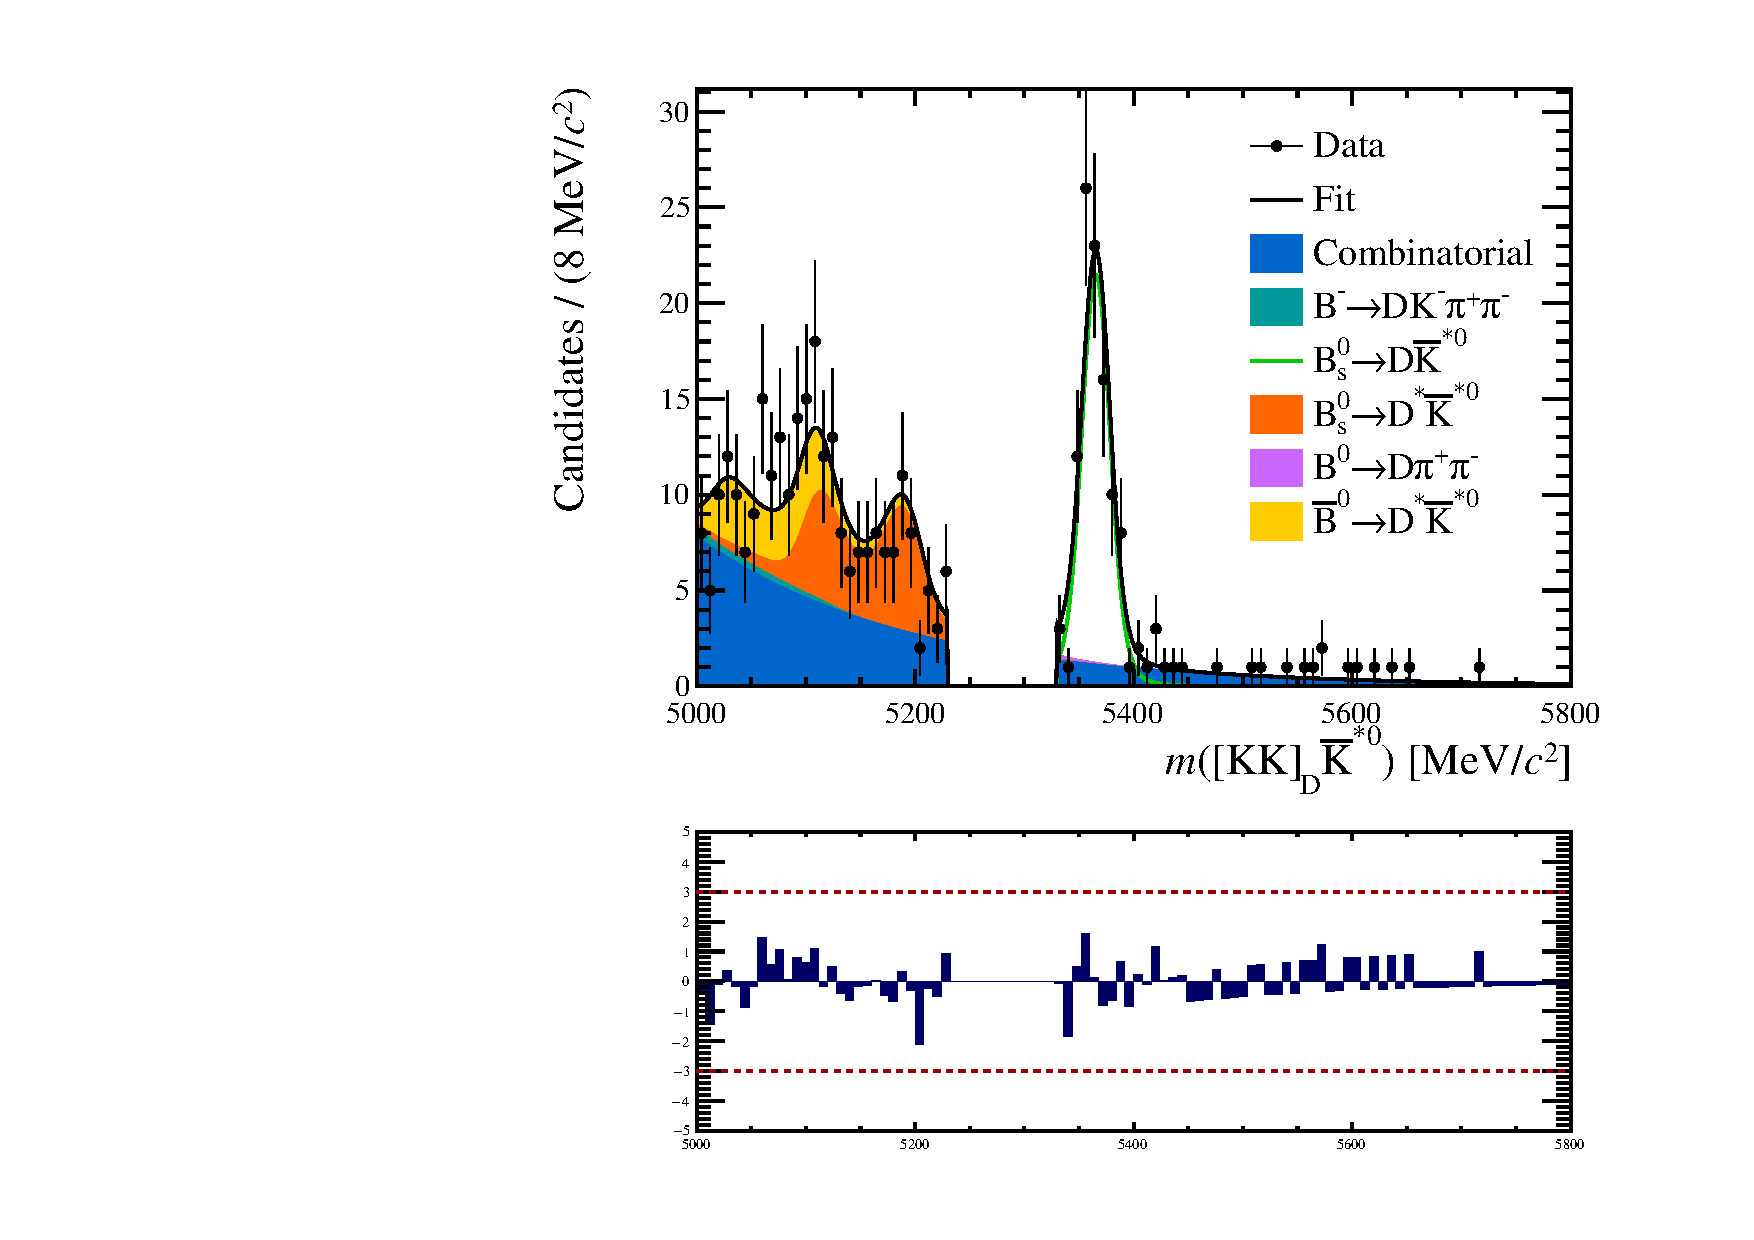
\includegraphics[width=0.45\textwidth]{ANA_resources/Plots/Data_fit/twoAndFourBody_data_split_KK_run1_minus.pdf}} \\
        \subfloat[][$B^0 \to D(KK)K^{*0}$ Run 2]{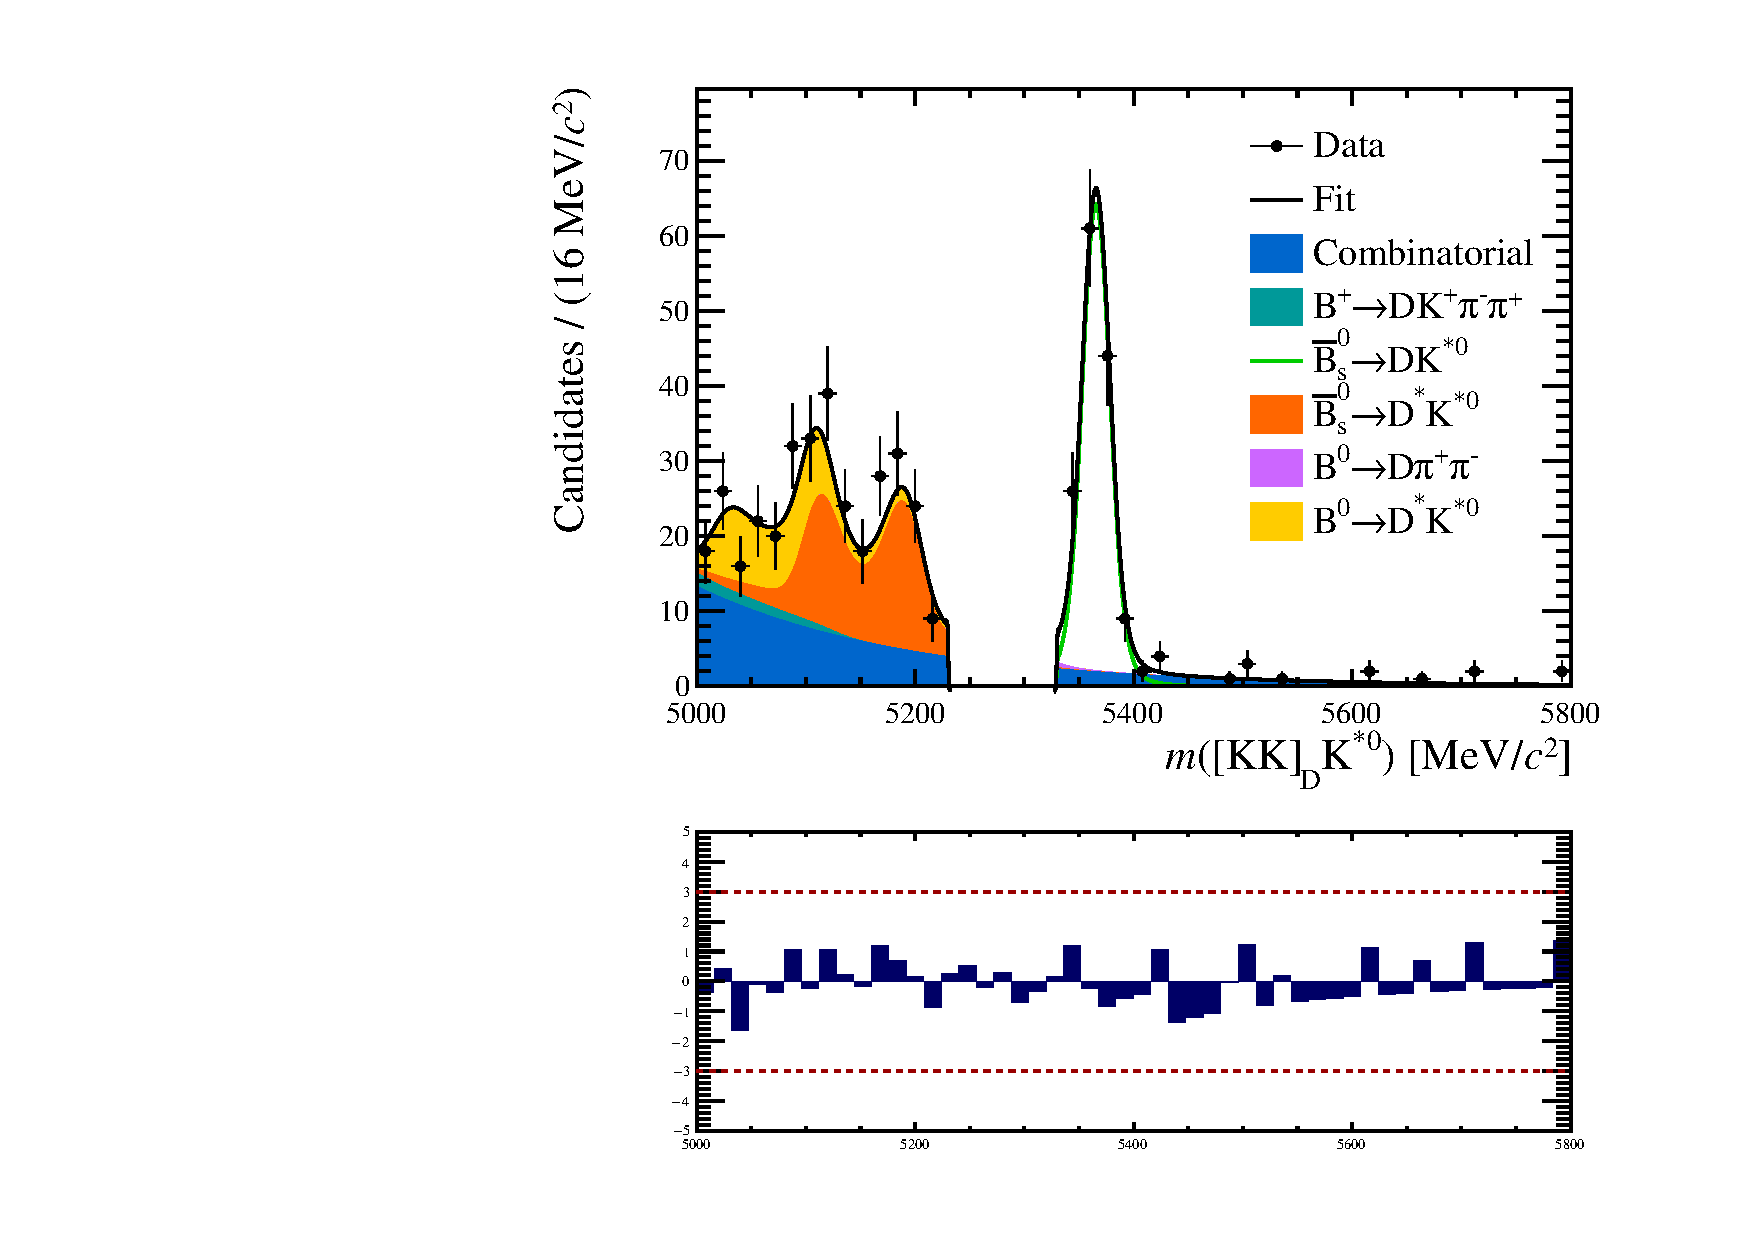
\includegraphics[width=0.45\textwidth]{ANA_resources/Plots/Data_fit/twoAndFourBody_data_split_KK_run2_plus.pdf}} &
        \subfloat[][$\bar{B}^0 \to D(KK)\bar{K}^{*0}$ Run 2]{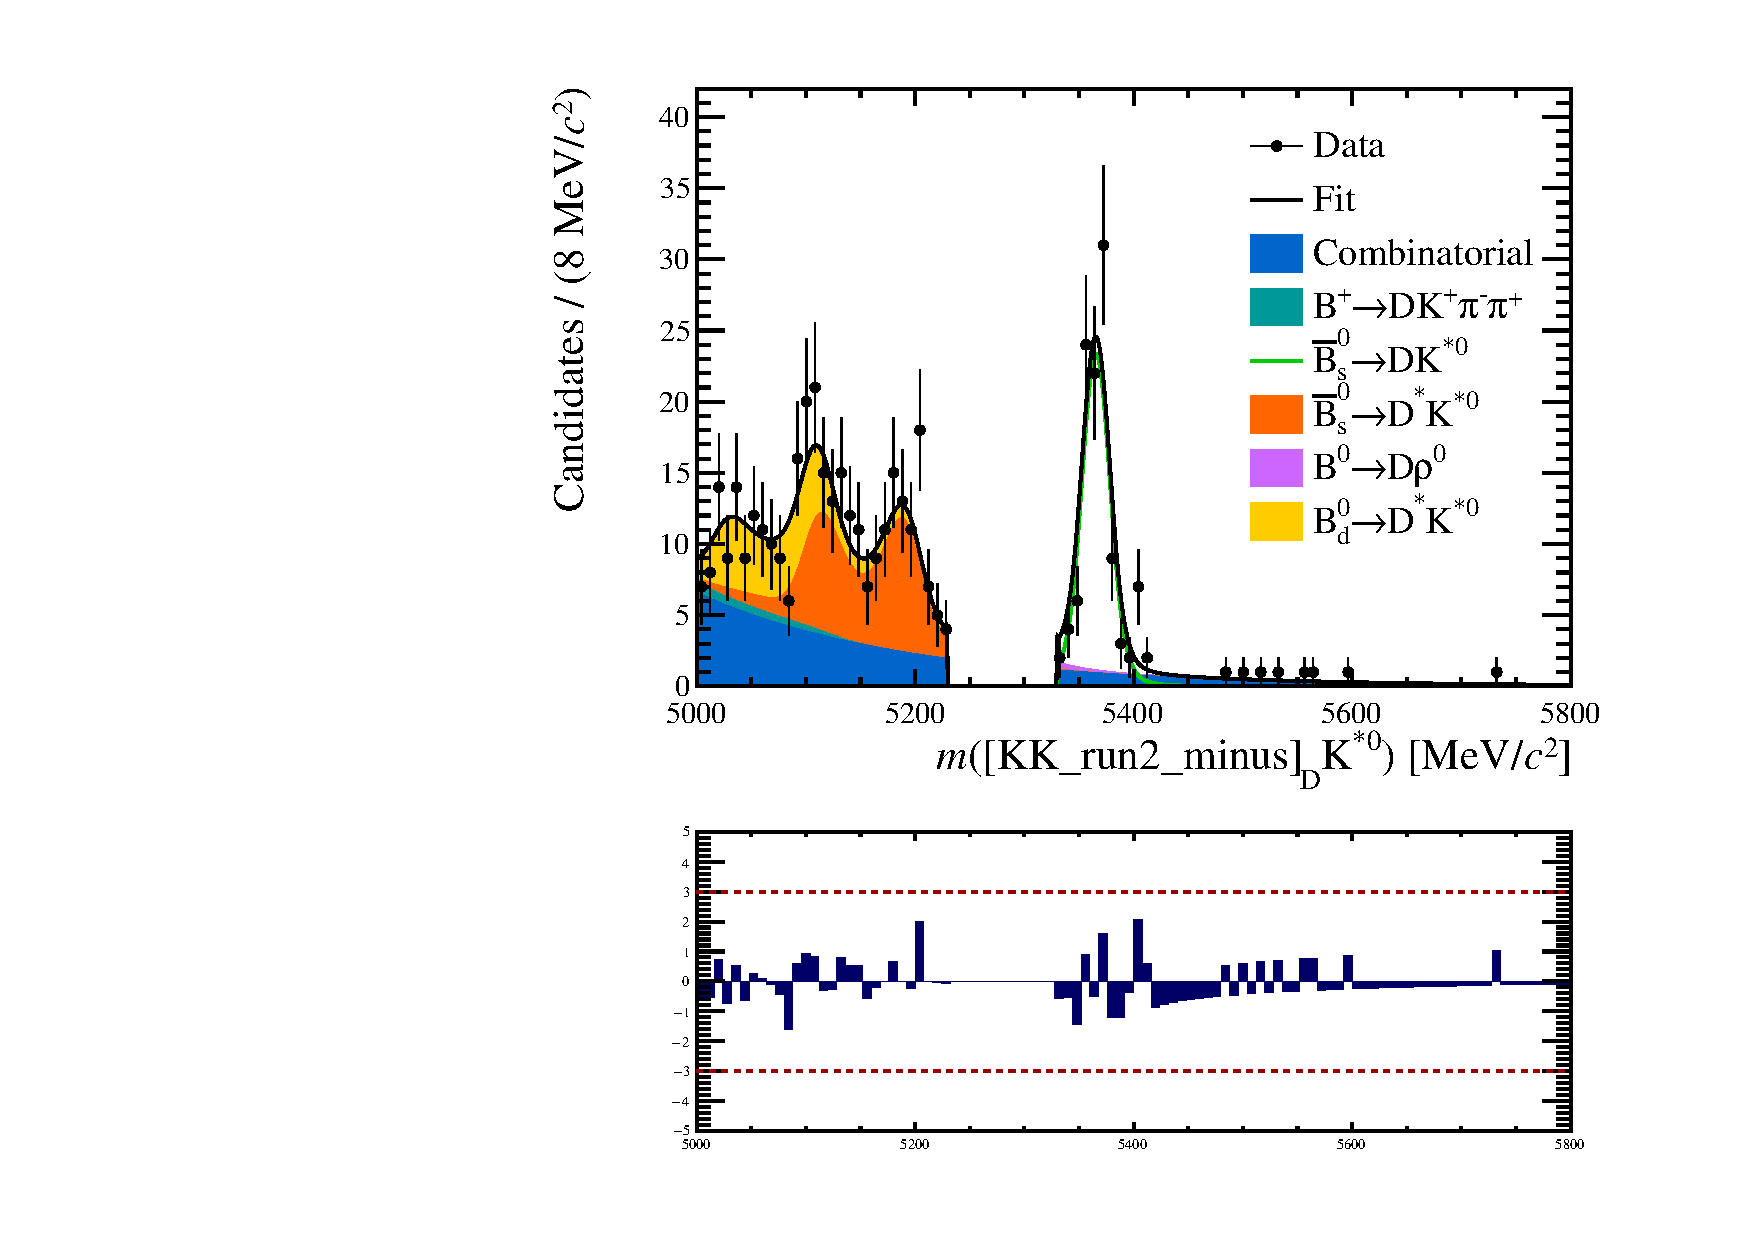
\includegraphics[width=0.45\textwidth]{ANA_resources/Plots/Data_fit/twoAndFourBody_data_split_KK_run2_minus.pdf}} \\
    \end{tabular}
    \caption{Fit to $B$ invariant mass of selected candidates in the $KK$ final state, split by $B$ flavour and run.}
\label{fig:data_fit_KK}
\end{figure}
\begin{figure}
    \centering
    \begin{tabular}{cc}
        \subfloat[][$B^0 \to D(\pi\pi)K^{*0}$ Run 1]{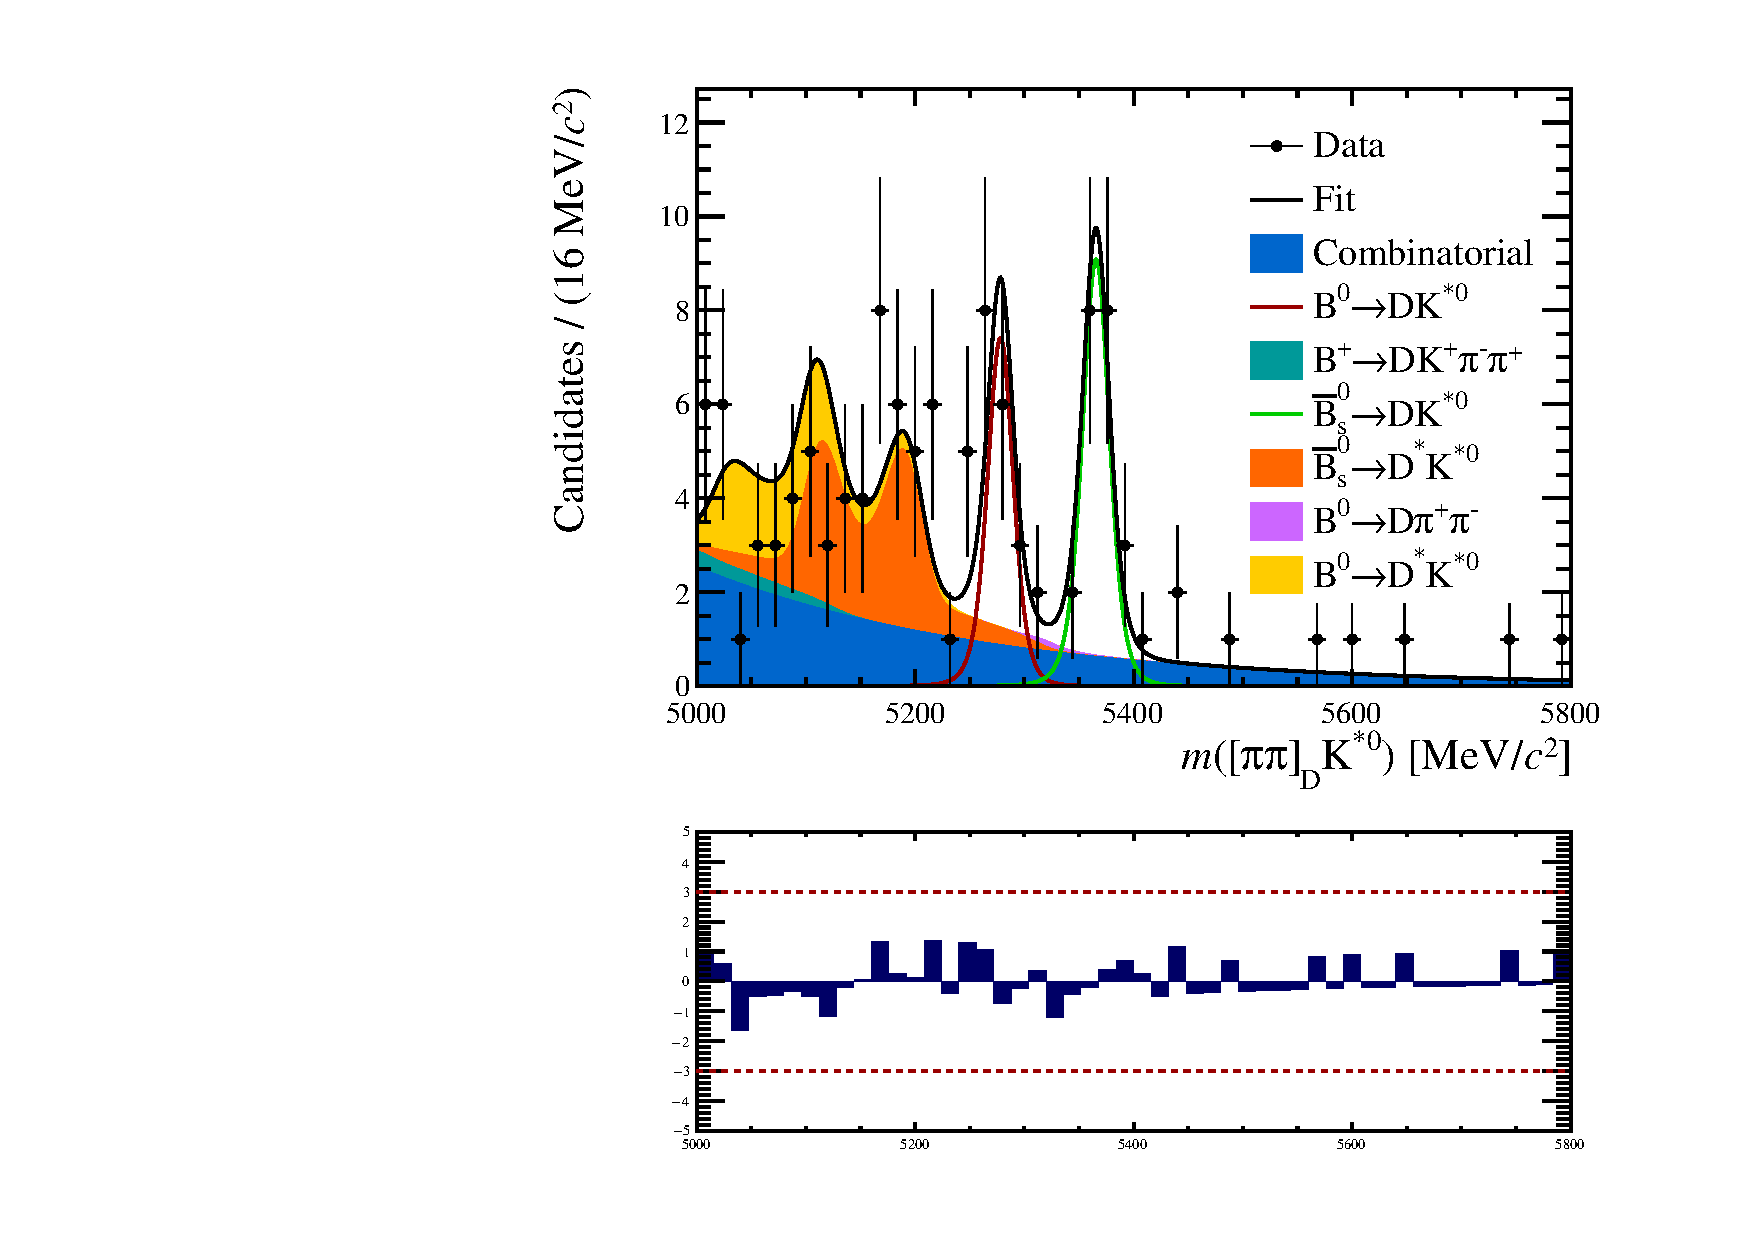
\includegraphics[width=0.45\textwidth]{ANA_resources/Plots/Data_fit/twoAndFourBody_data_split_pipi_run1_plus.pdf}} &
        \subfloat[][$\bar{B}^0 \to D(\pi\pi)\bar{K}^{*0}$ Run 1]{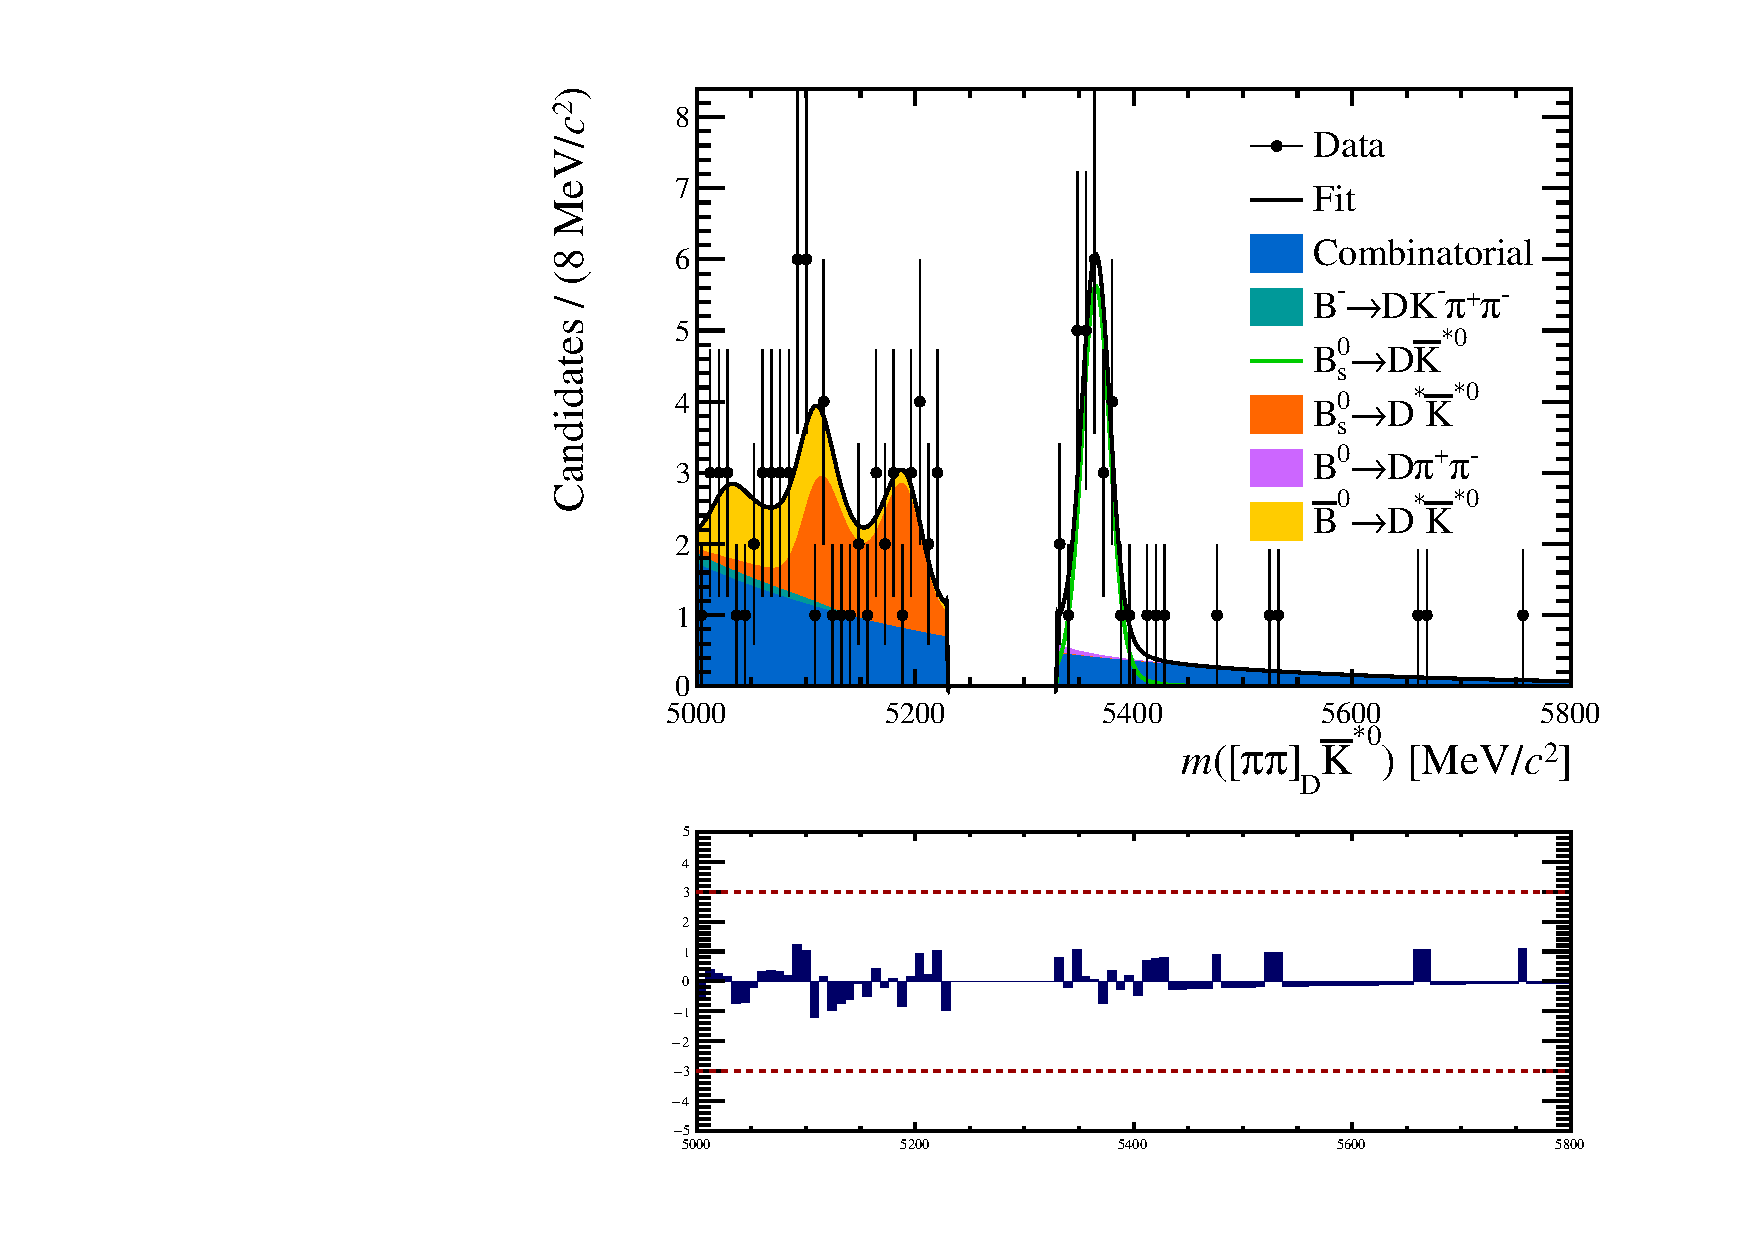
\includegraphics[width=0.45\textwidth]{ANA_resources/Plots/Data_fit/twoAndFourBody_data_split_pipi_run1_minus.pdf}} \\
        \subfloat[][$B^0 \to D(\pi\pi)K^{*0}$ Run 2]{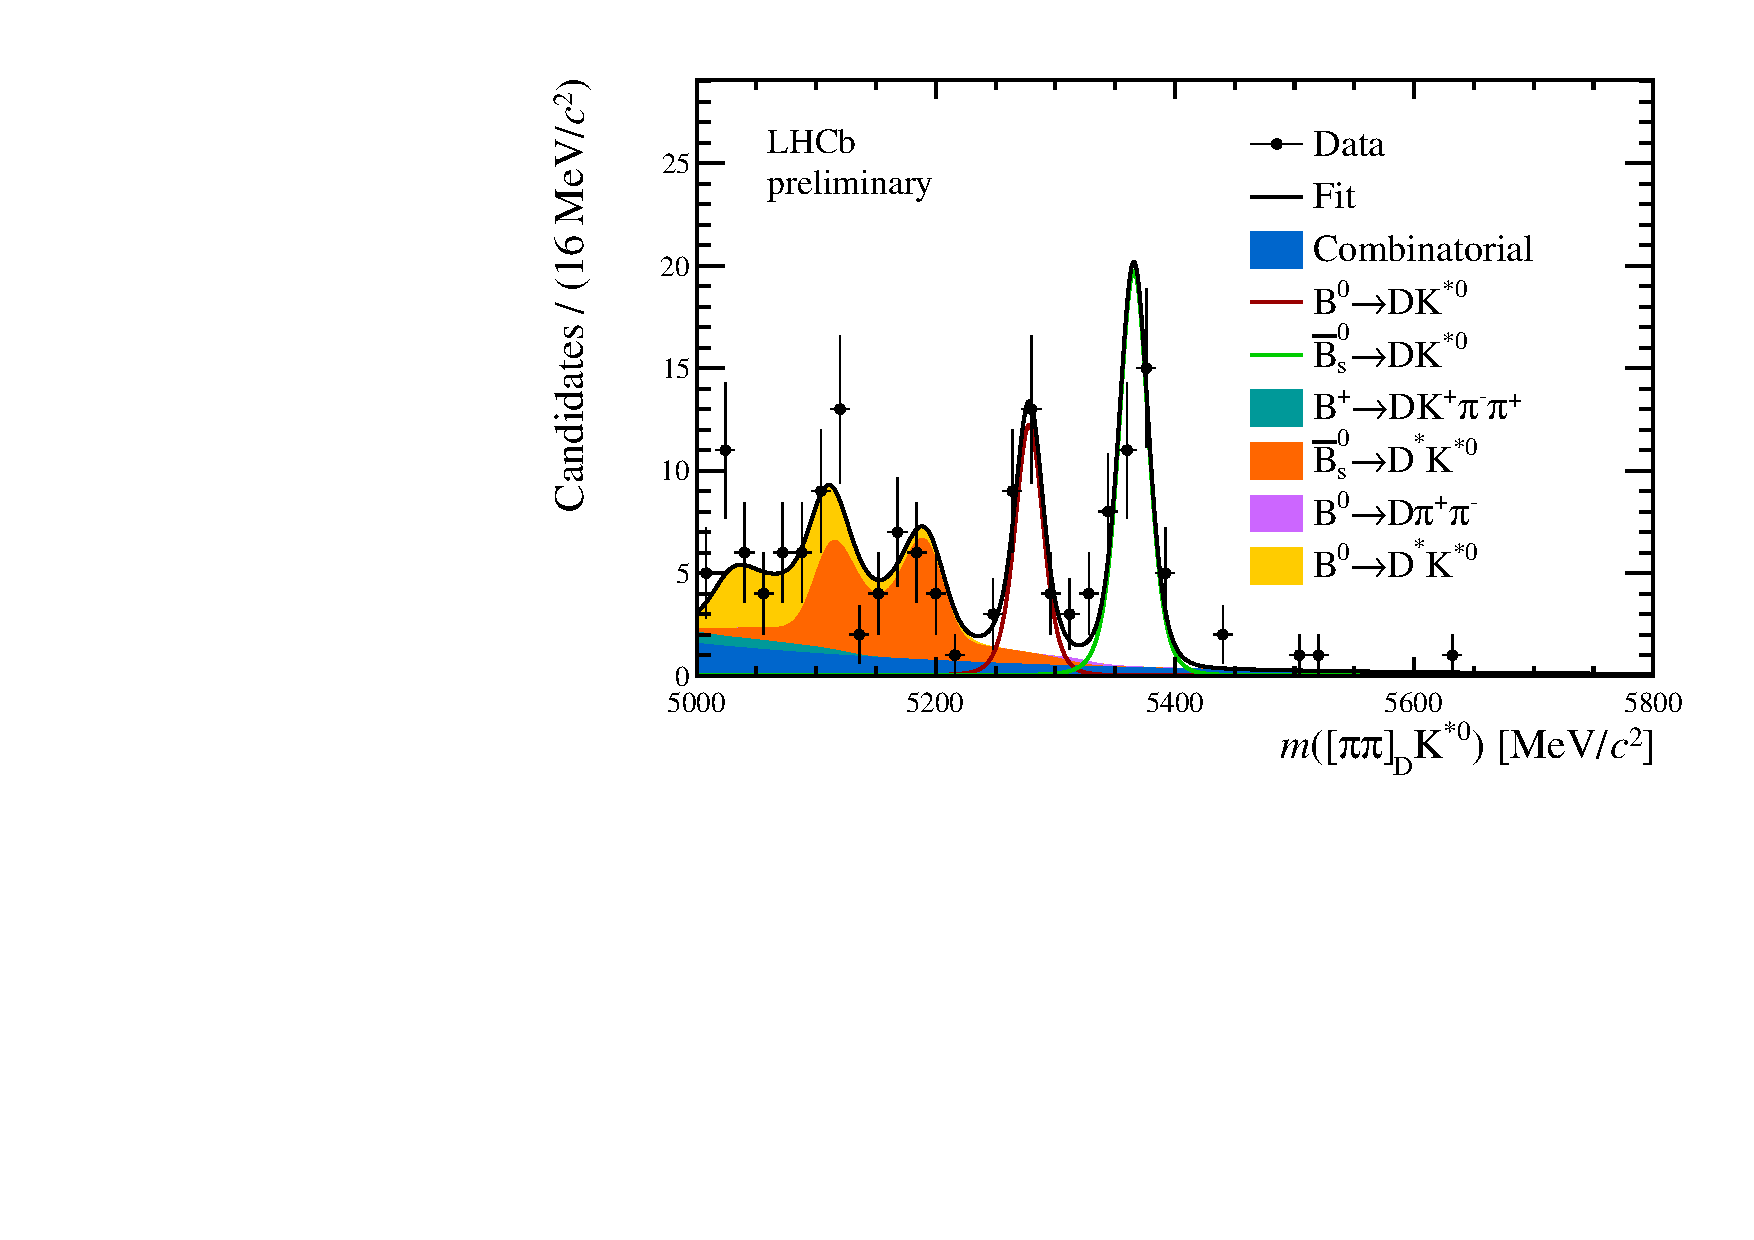
\includegraphics[width=0.45\textwidth]{ANA_resources/Plots/Data_fit/twoAndFourBody_data_split_pipi_run2_plus.pdf}} &
        \subfloat[][$\bar{B}^0 \to D(\pi\pi)\bar{K}^{*0}$ Run 2]{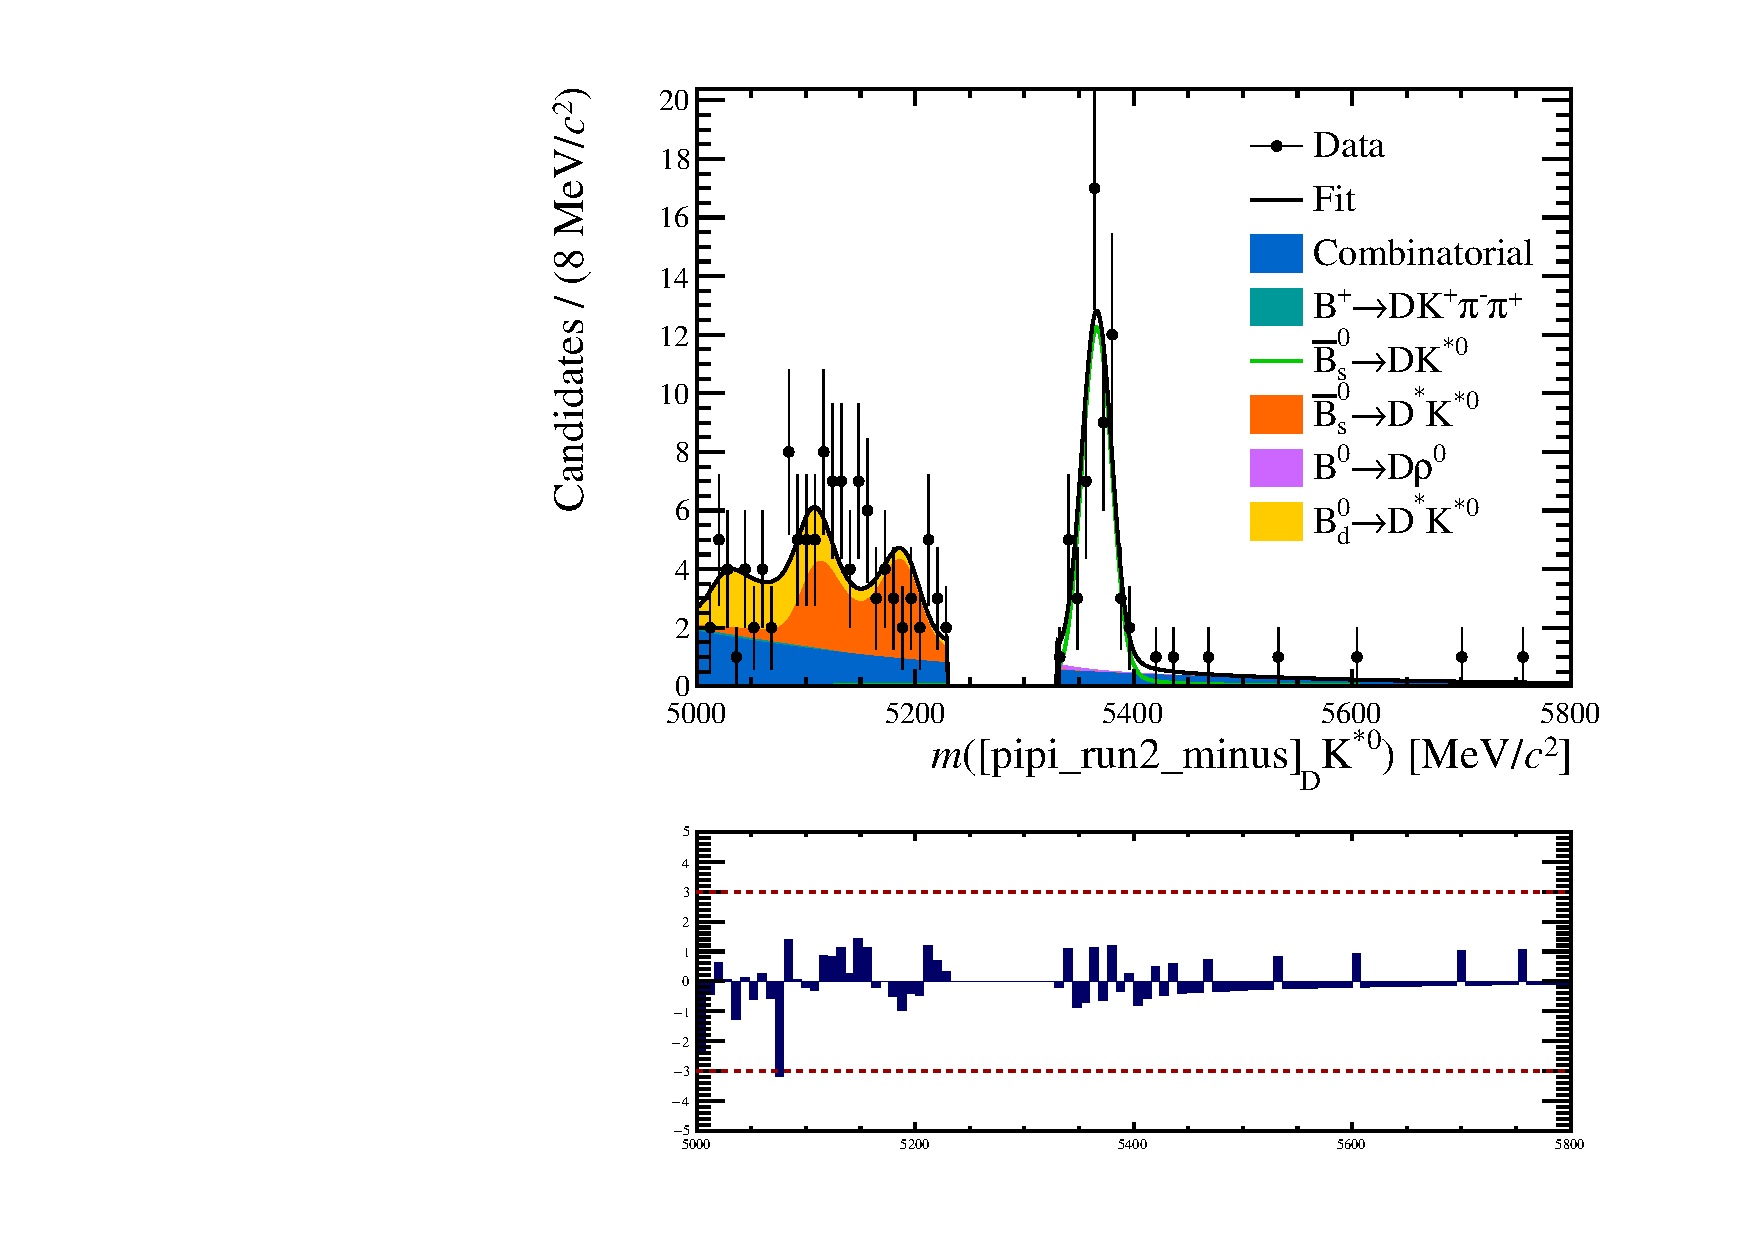
\includegraphics[width=0.45\textwidth]{ANA_resources/Plots/Data_fit/twoAndFourBody_data_split_pipi_run2_minus.pdf}} \\
    \end{tabular}
    \caption{Fit to $B$ invariant mass of selected candidates in the $\pi\pi$ final state, split by $B$ flavour and run.}
\label{fig:data_fit_pipi}
\end{figure}
\begin{figure}
    \centering
    \begin{tabular}{cc}
        \subfloat[][$B^0 \to D(K\pi\pi\pi)K^{*0}$ Run 1]{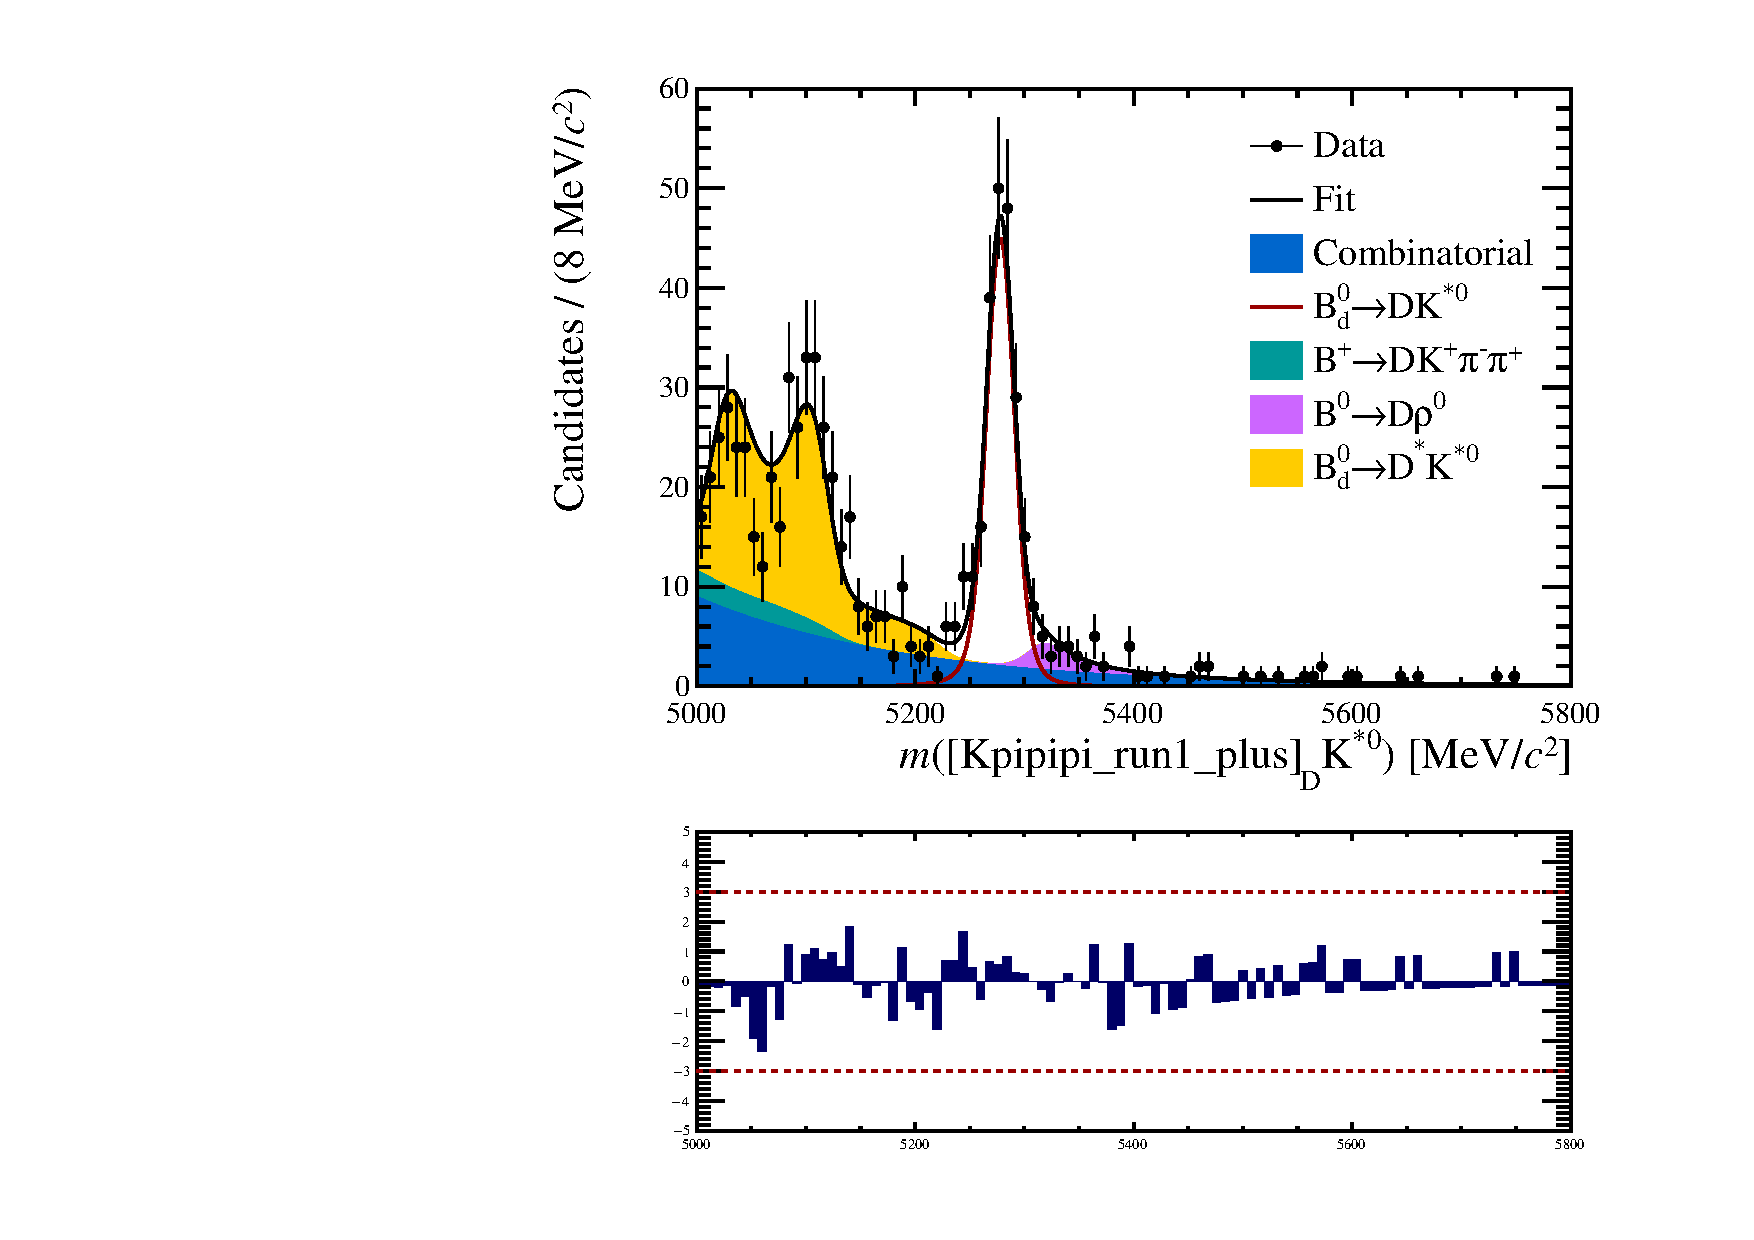
\includegraphics[width=0.45\textwidth]{ANA_resources/Plots/Data_fit/twoAndFourBody_data_split_Kpipipi_run1_plus.pdf}} &
        \subfloat[][$\bar{B}^0 \to D(K\pi\pi\pi)\bar{K}^{*0}$ Run 1]{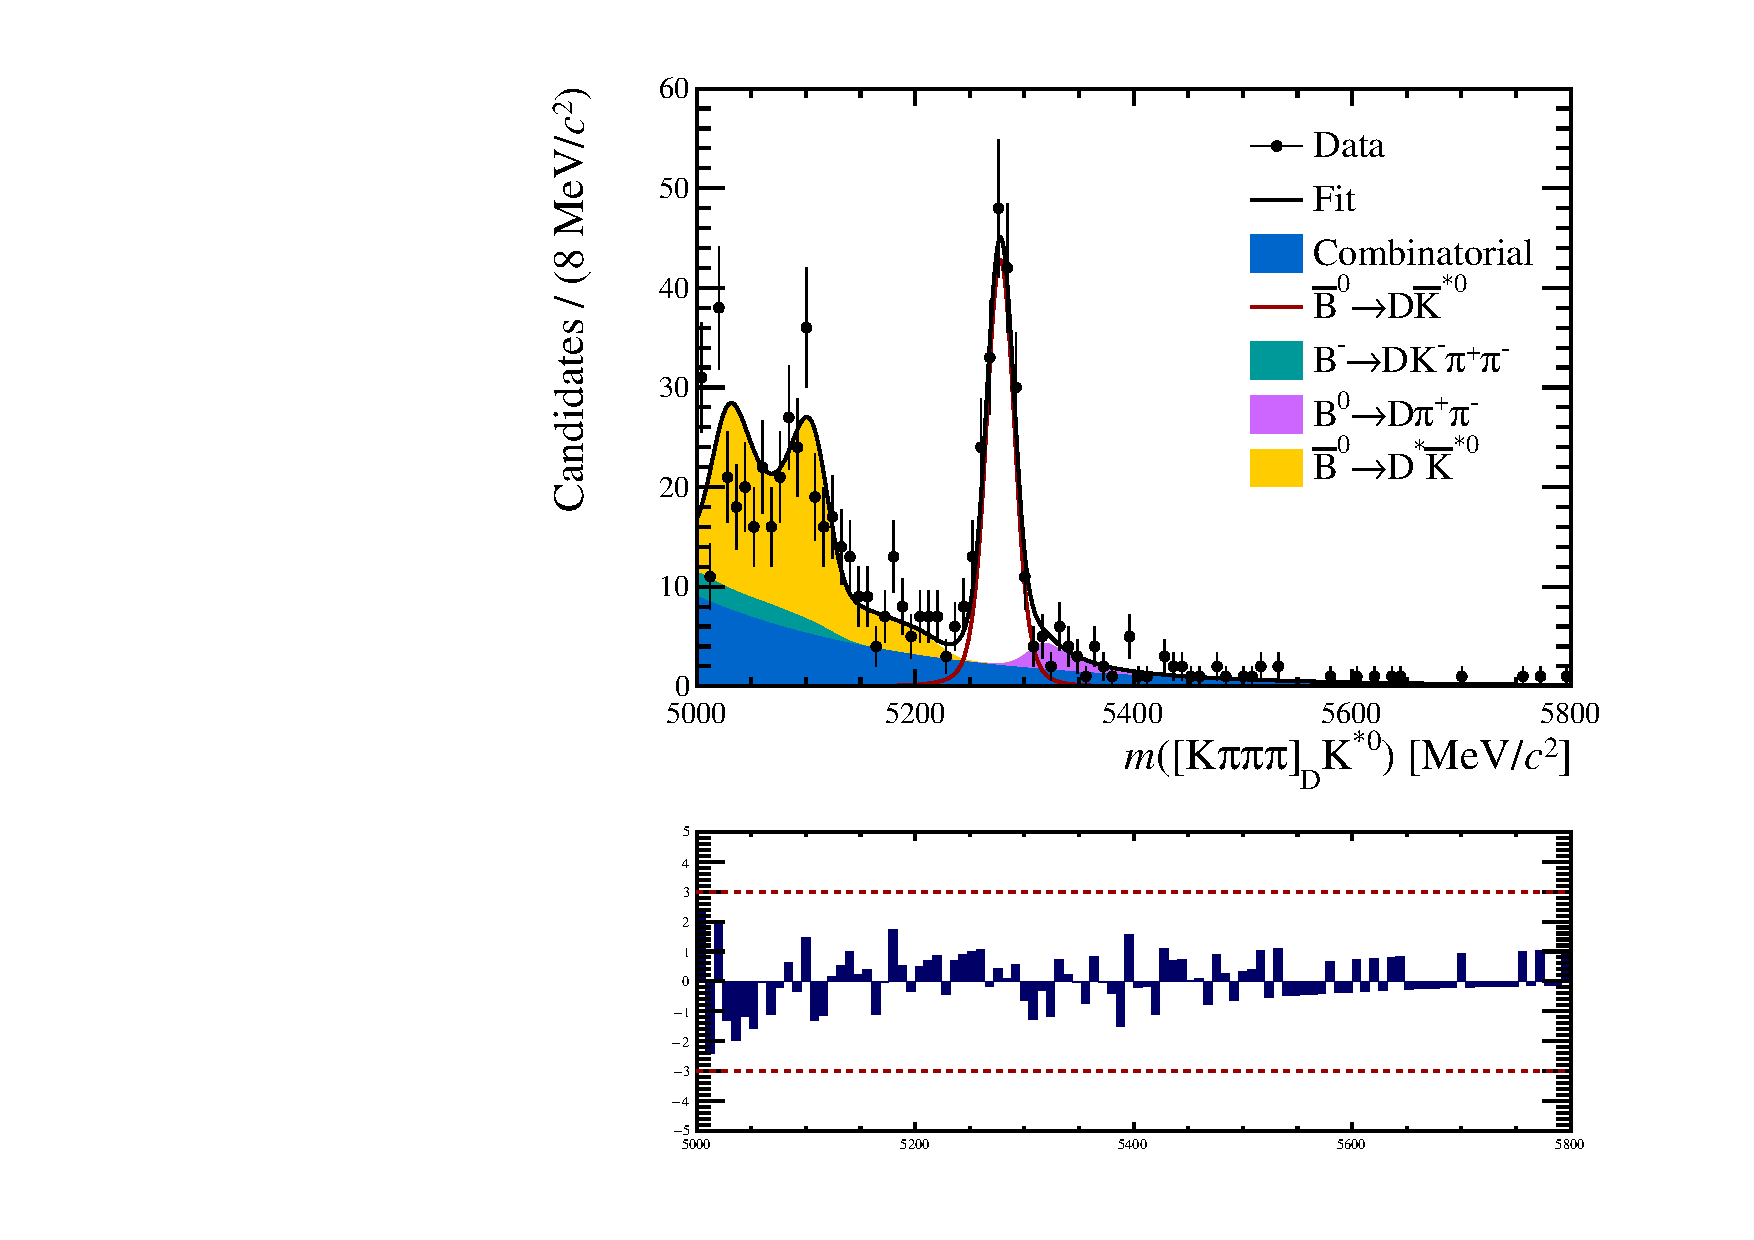
\includegraphics[width=0.45\textwidth]{ANA_resources/Plots/Data_fit/twoAndFourBody_data_split_Kpipipi_run1_minus.pdf}} \\
        \subfloat[][$B^0 \to D(K\pi\pi\pi)K^{*0}$ Run 2]{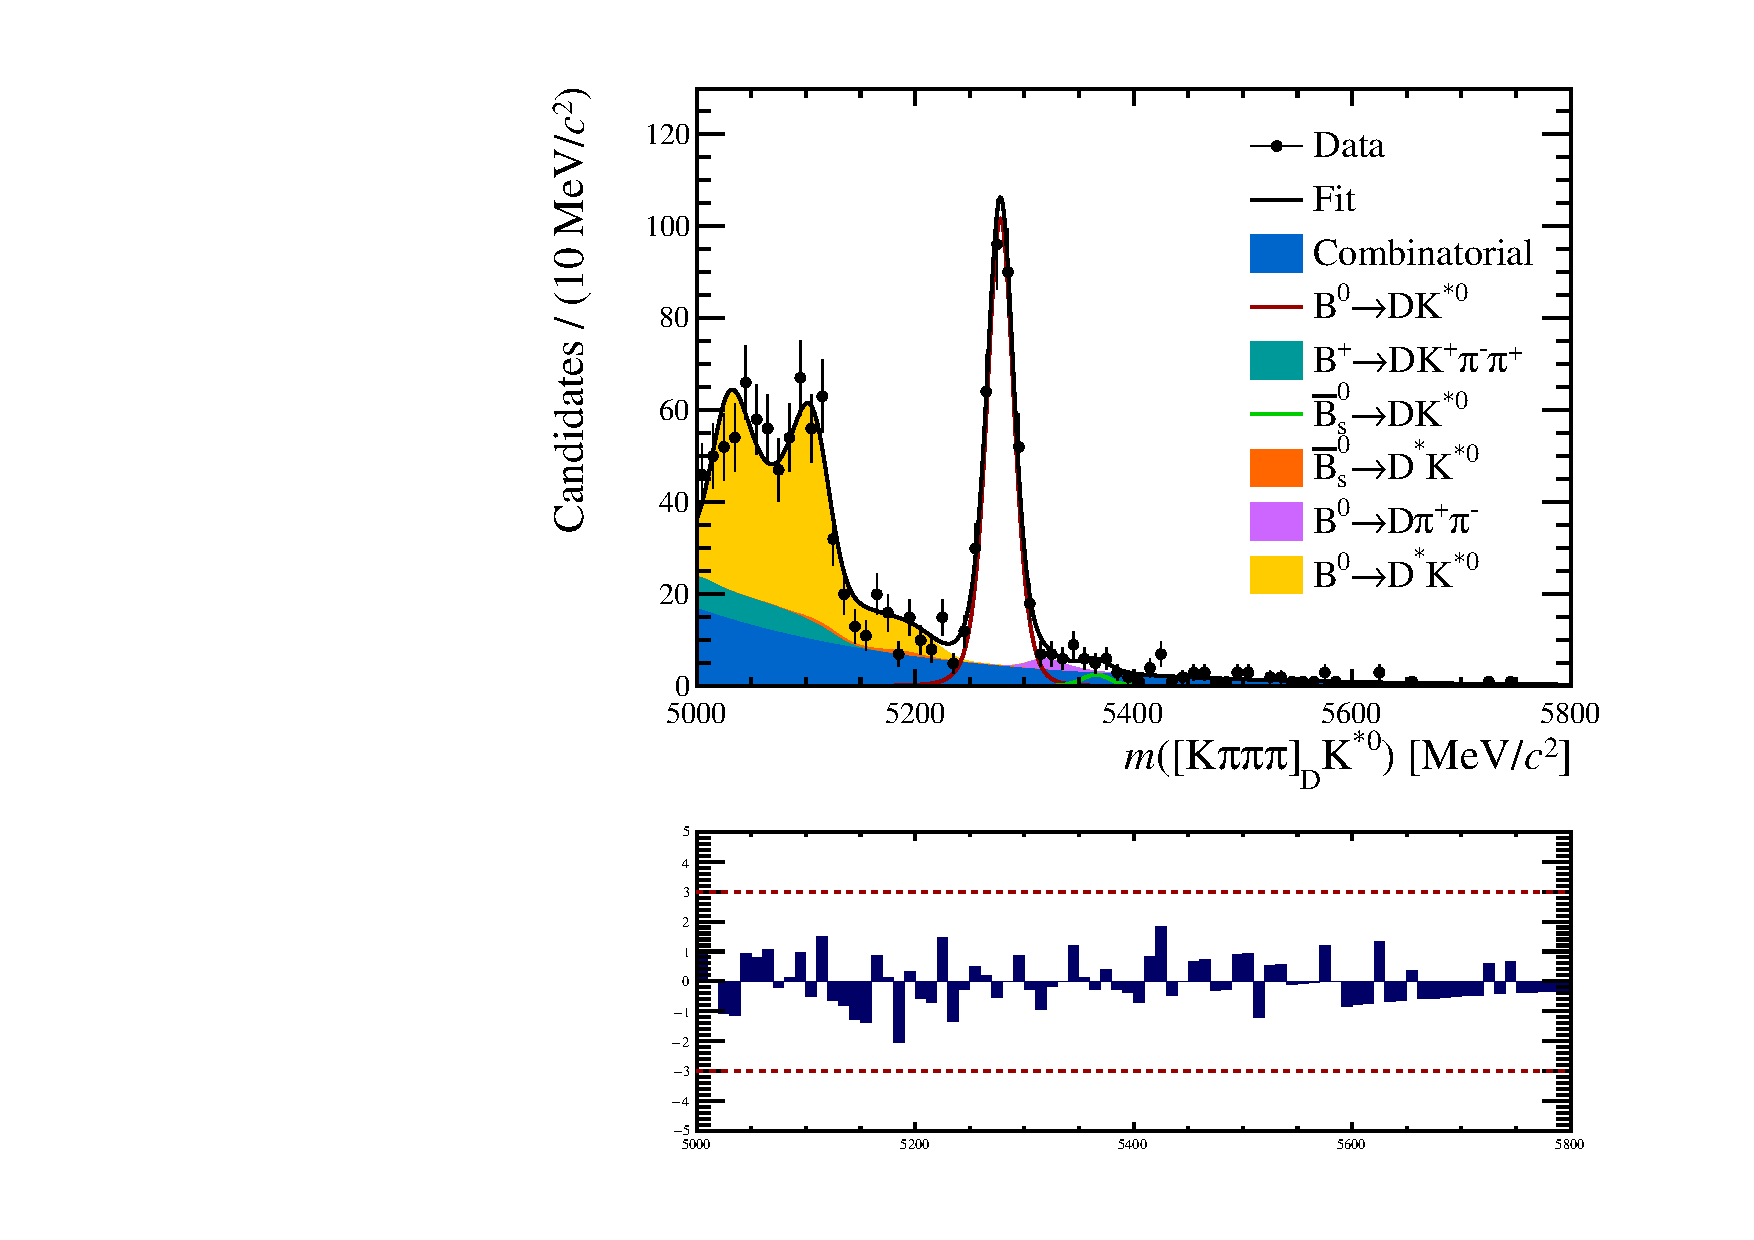
\includegraphics[width=0.45\textwidth]{ANA_resources/Plots/Data_fit/twoAndFourBody_data_split_Kpipipi_run2_plus.pdf}} &
        \subfloat[][$\bar{B}^0 \to D(K\pi\pi\pi)\bar{K}^{*0}$ Run 2]{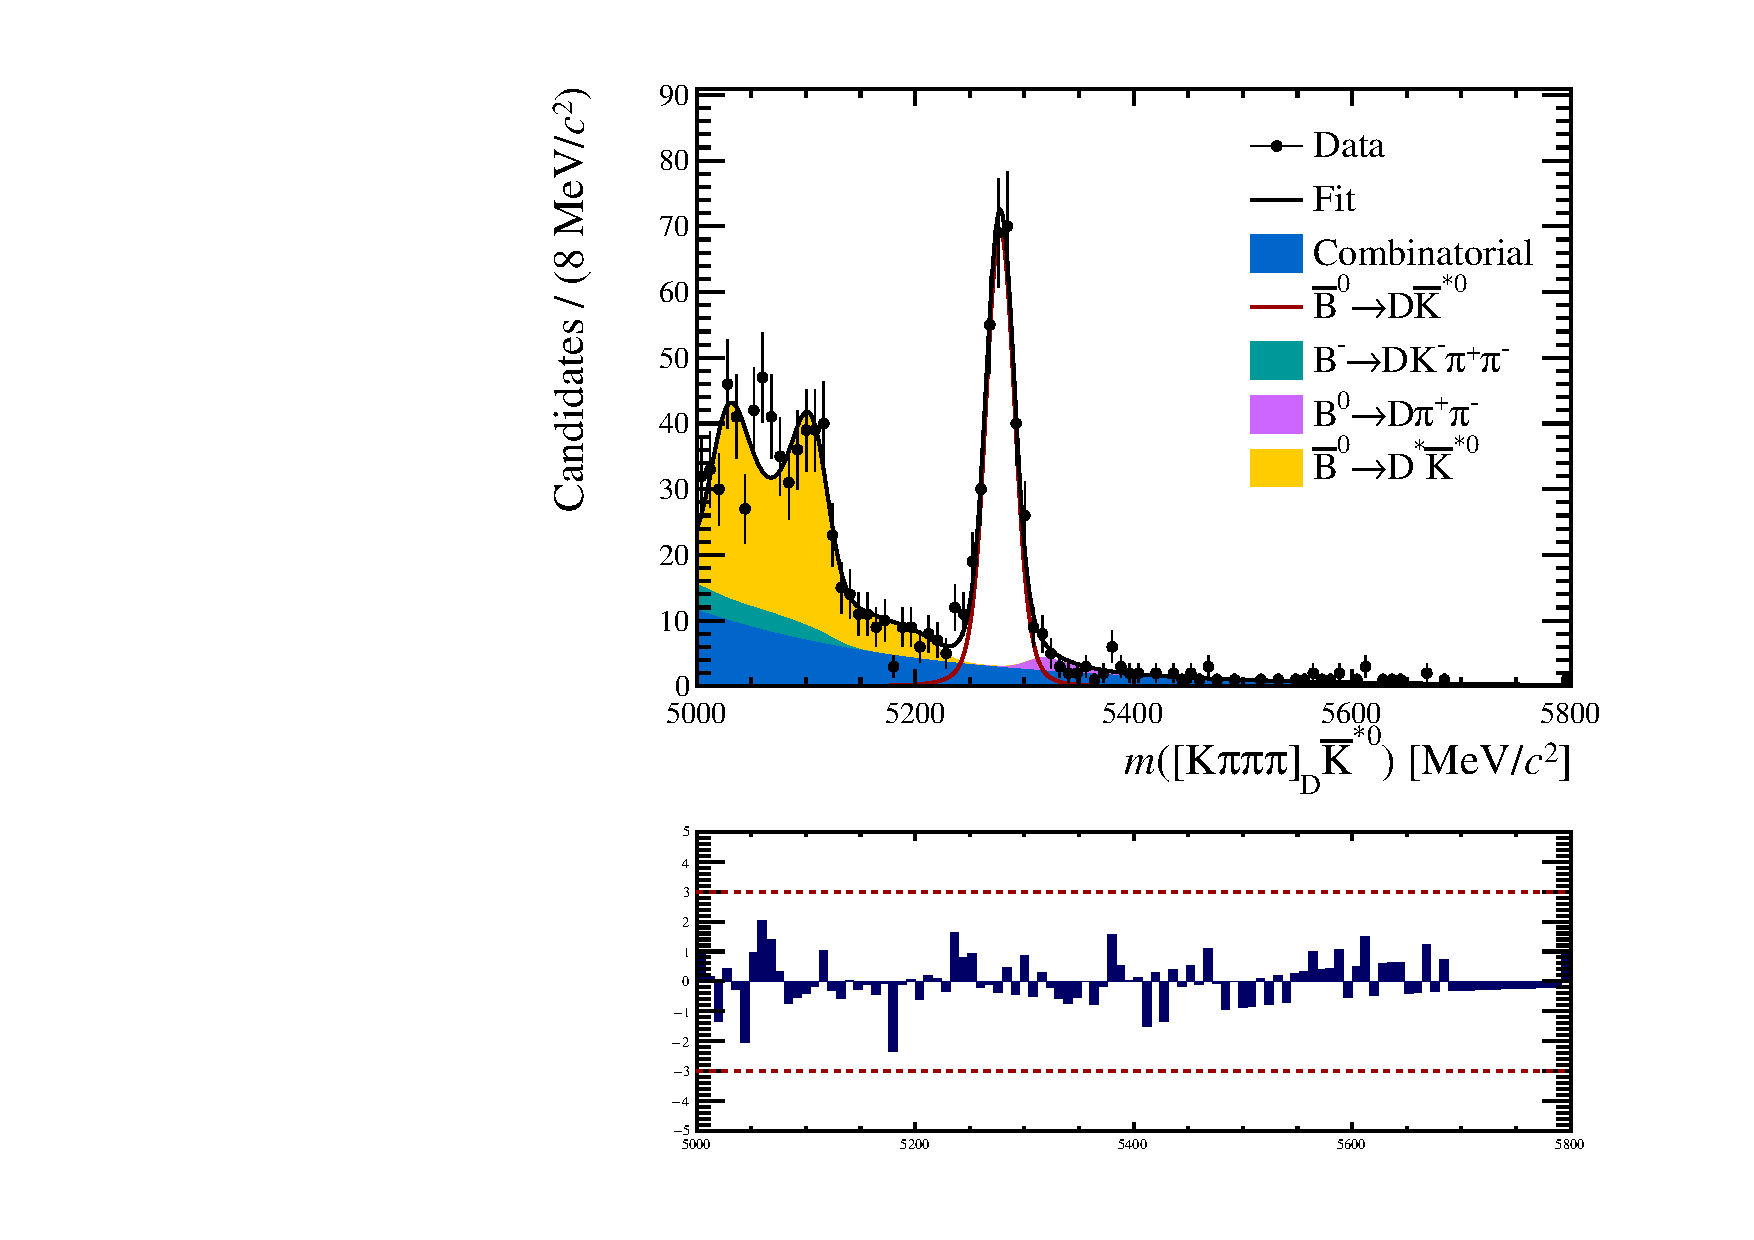
\includegraphics[width=0.45\textwidth]{ANA_resources/Plots/Data_fit/twoAndFourBody_data_split_Kpipipi_run2_minus.pdf}} \\
    \end{tabular}
    \caption{Fit to $B$ invariant mass of selected candidates in the $K\pi\pi\pi$ final state, split by $B$ flavour and run.}
\label{fig:data_fit_Kpipipi}
\end{figure}
\begin{figure}
    \centering
    \begin{tabular}{cc}
        \subfloat[][$B^0 \to D(\pi K\pi\pi)K^{*0}$ Run 1]{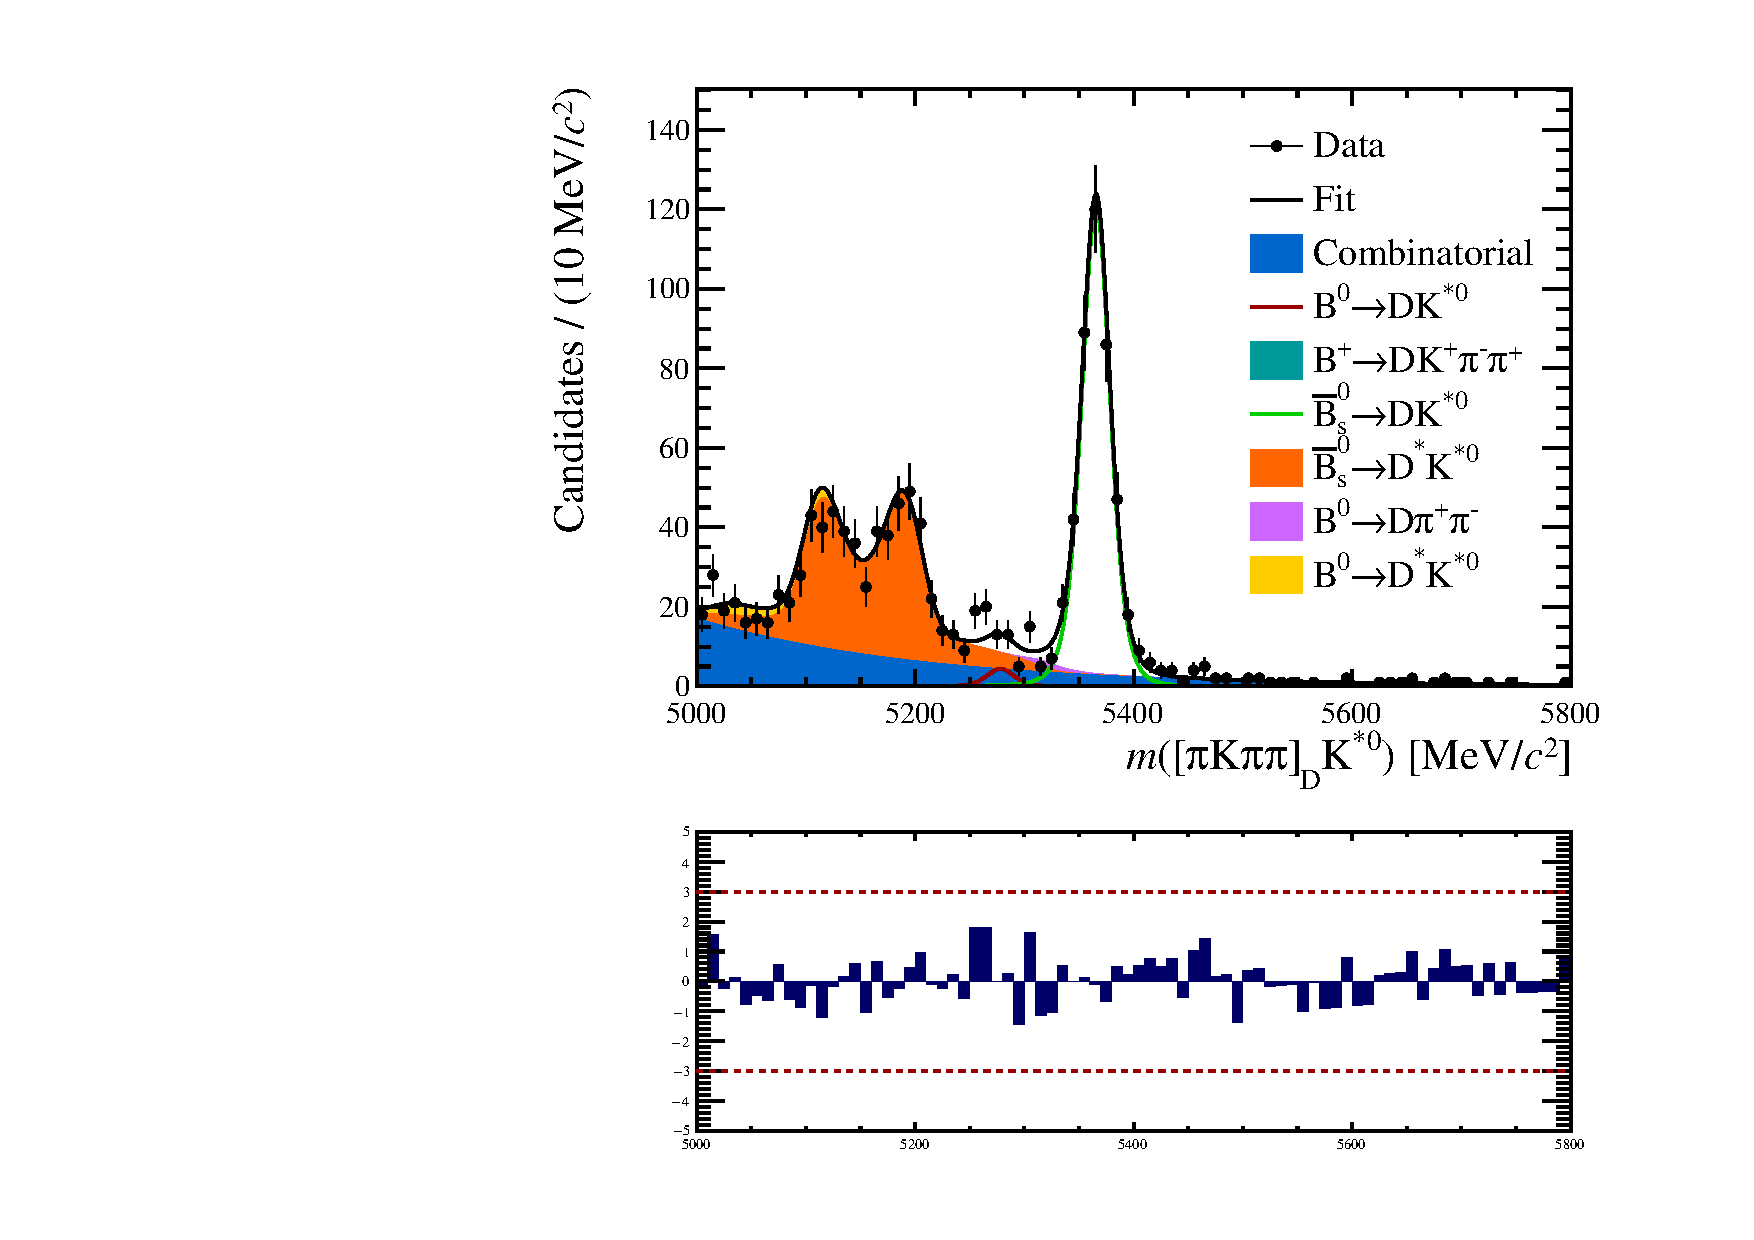
\includegraphics[width=0.45\textwidth]{ANA_resources/Plots/Data_fit/twoAndFourBody_data_split_piKpipi_run1_plus.pdf}} &
        \subfloat[][$\bar{B}^0 \to D(\pi K\pi\pi)\bar{K}^{*0}$ Run 1]{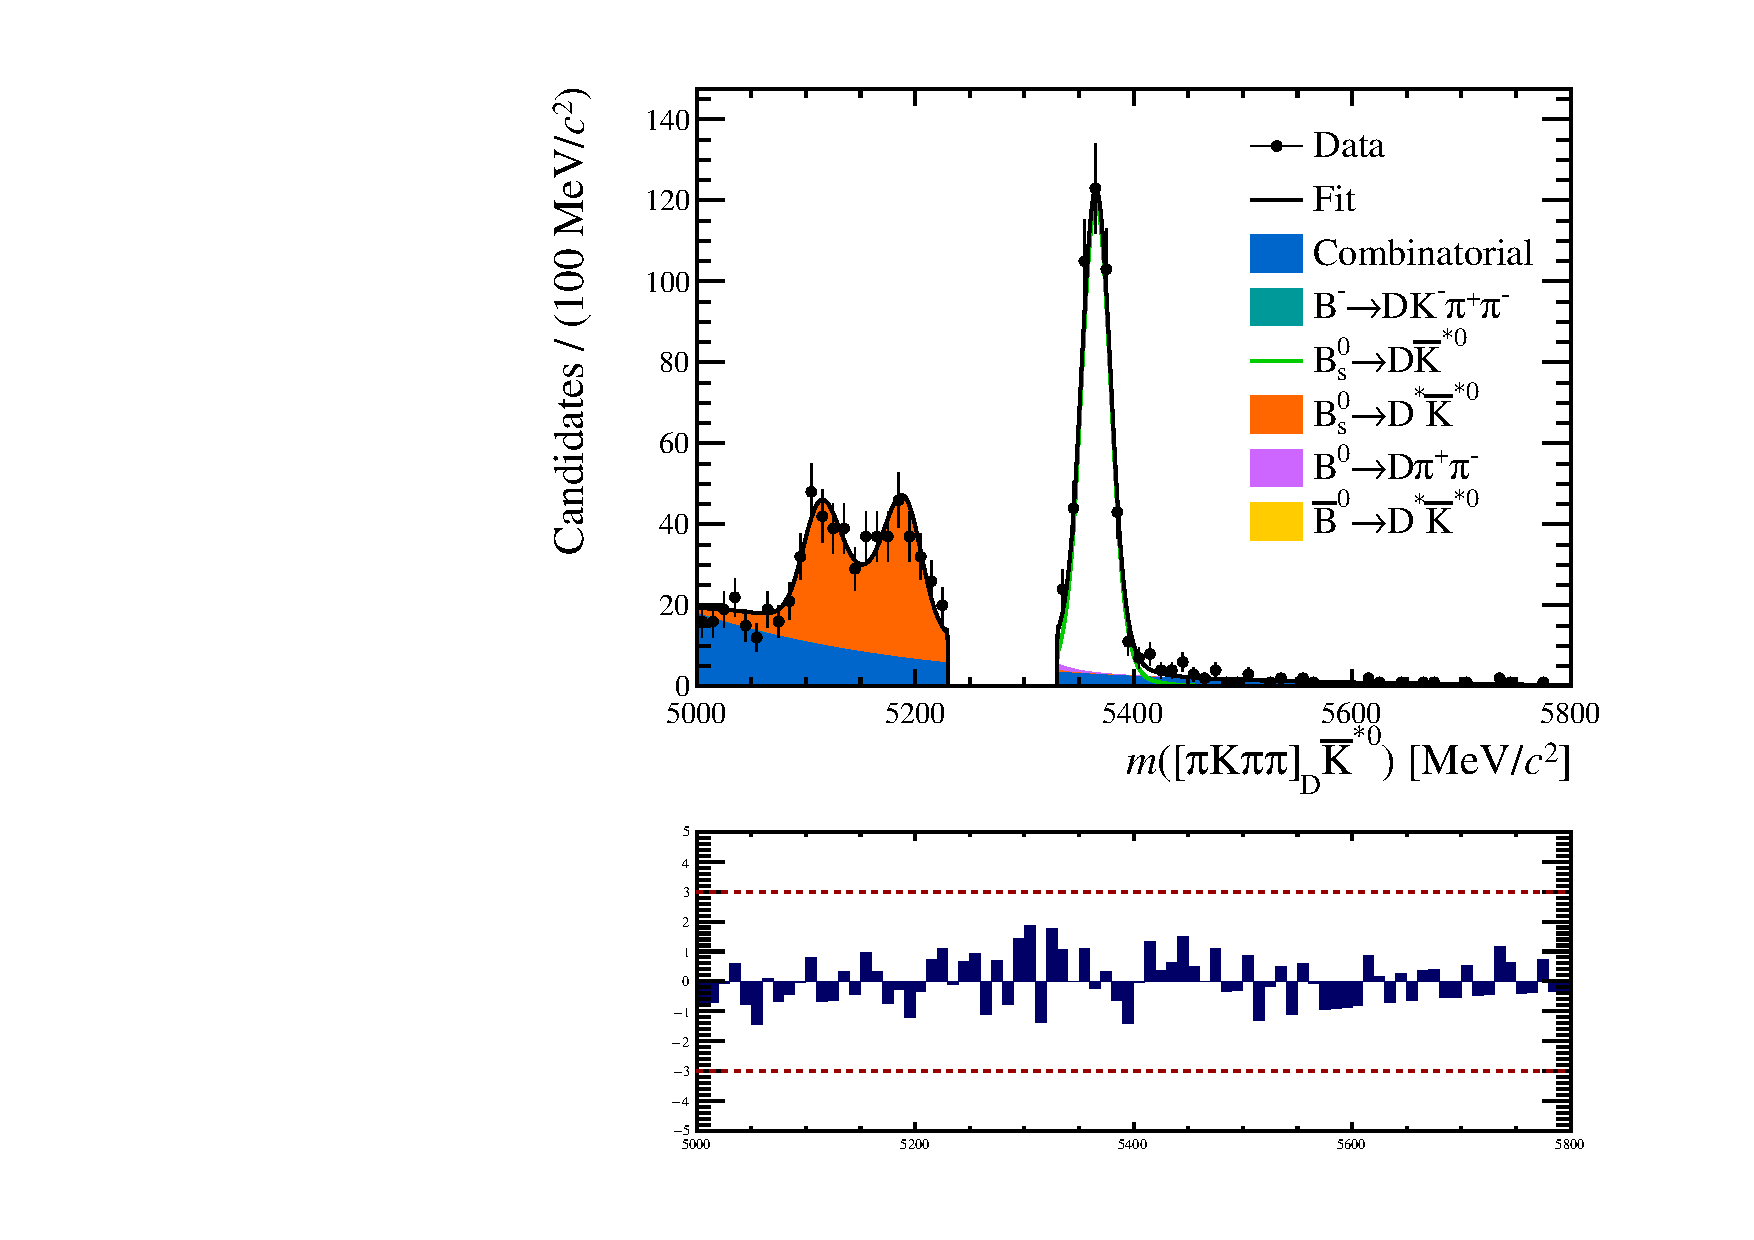
\includegraphics[width=0.45\textwidth]{ANA_resources/Plots/Data_fit/twoAndFourBody_data_split_piKpipi_run1_minus.pdf}} \\
        \subfloat[][$B^0 \to D(\pi K\pi\pi)K^{*0}$ Run 2]{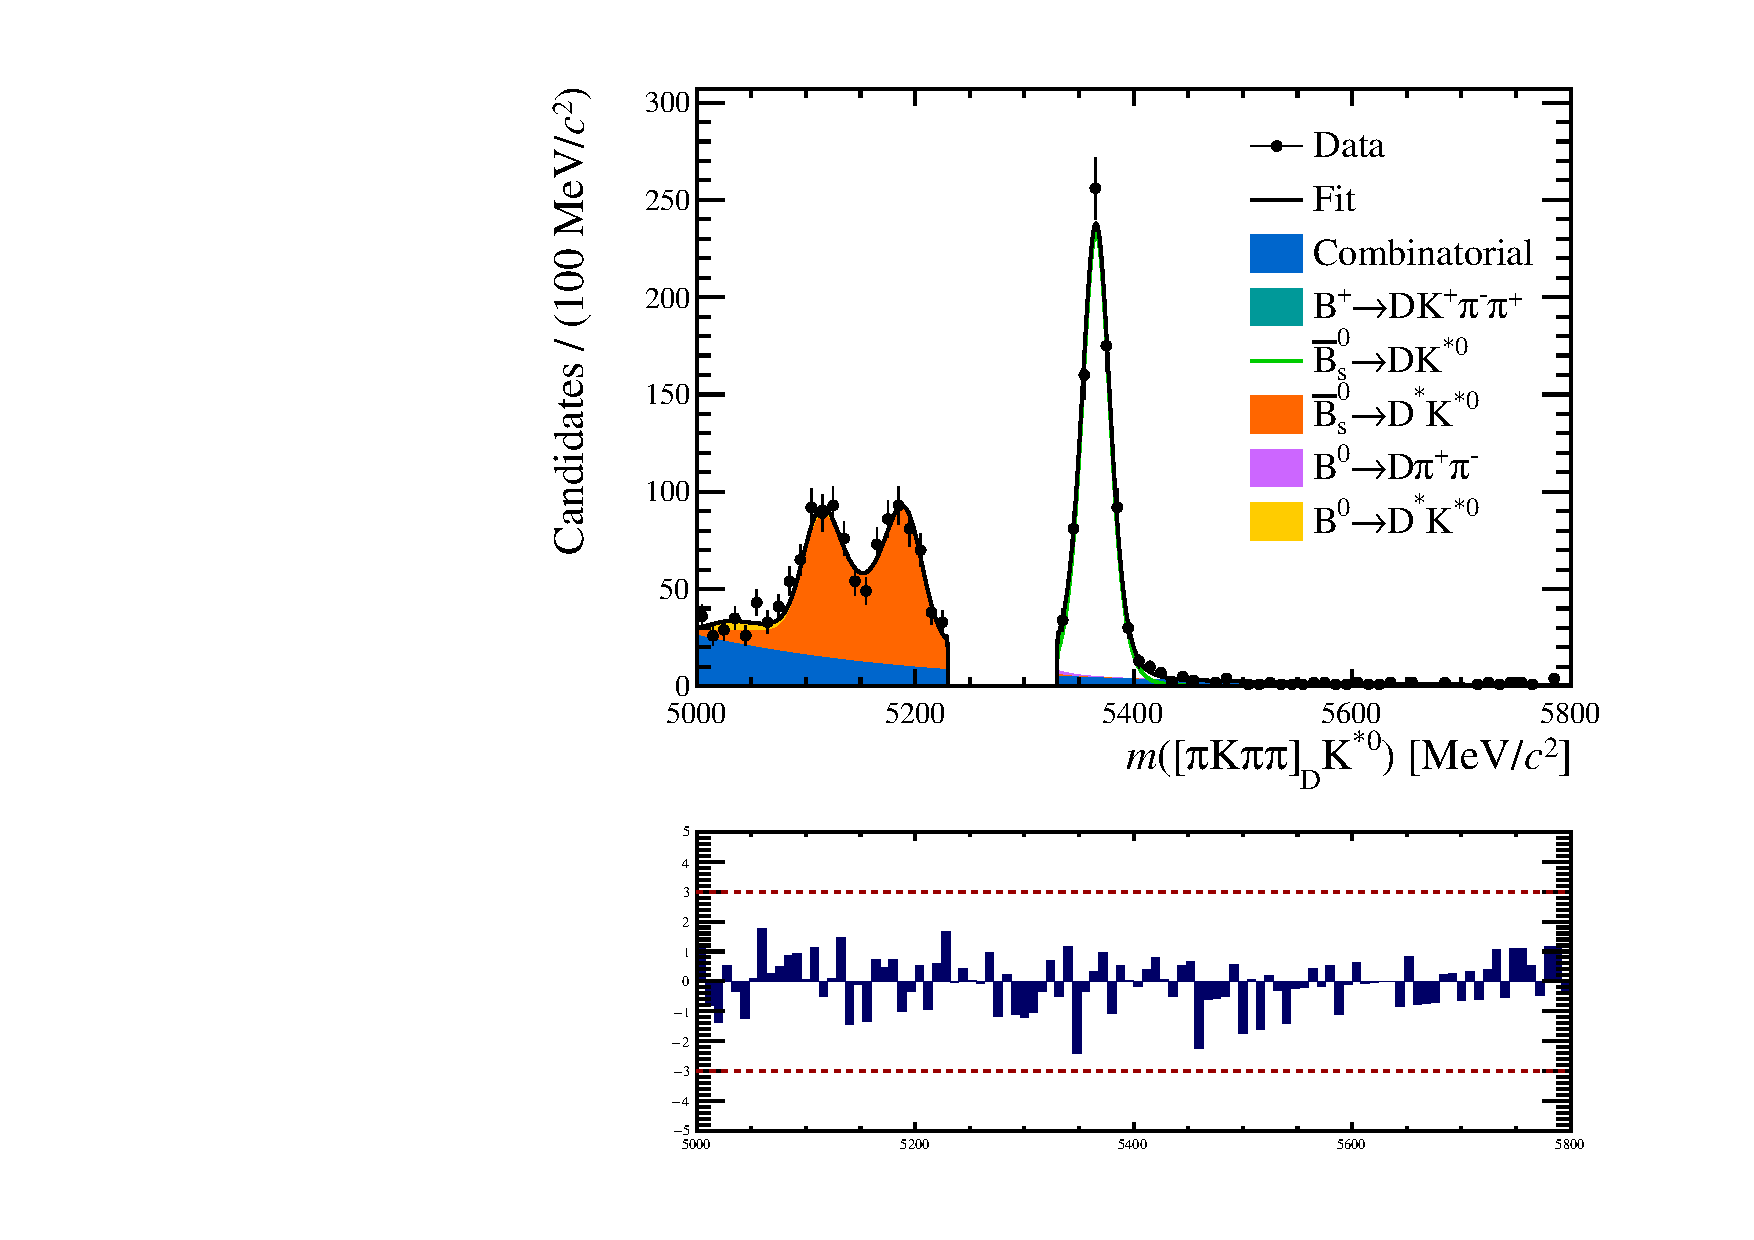
\includegraphics[width=0.45\textwidth]{ANA_resources/Plots/Data_fit/twoAndFourBody_data_split_piKpipi_run2_plus.pdf}} &
        \subfloat[][$\bar{B}^0 \to D(\pi K\pi\pi)\bar{K}^{*0}$ Run 2]{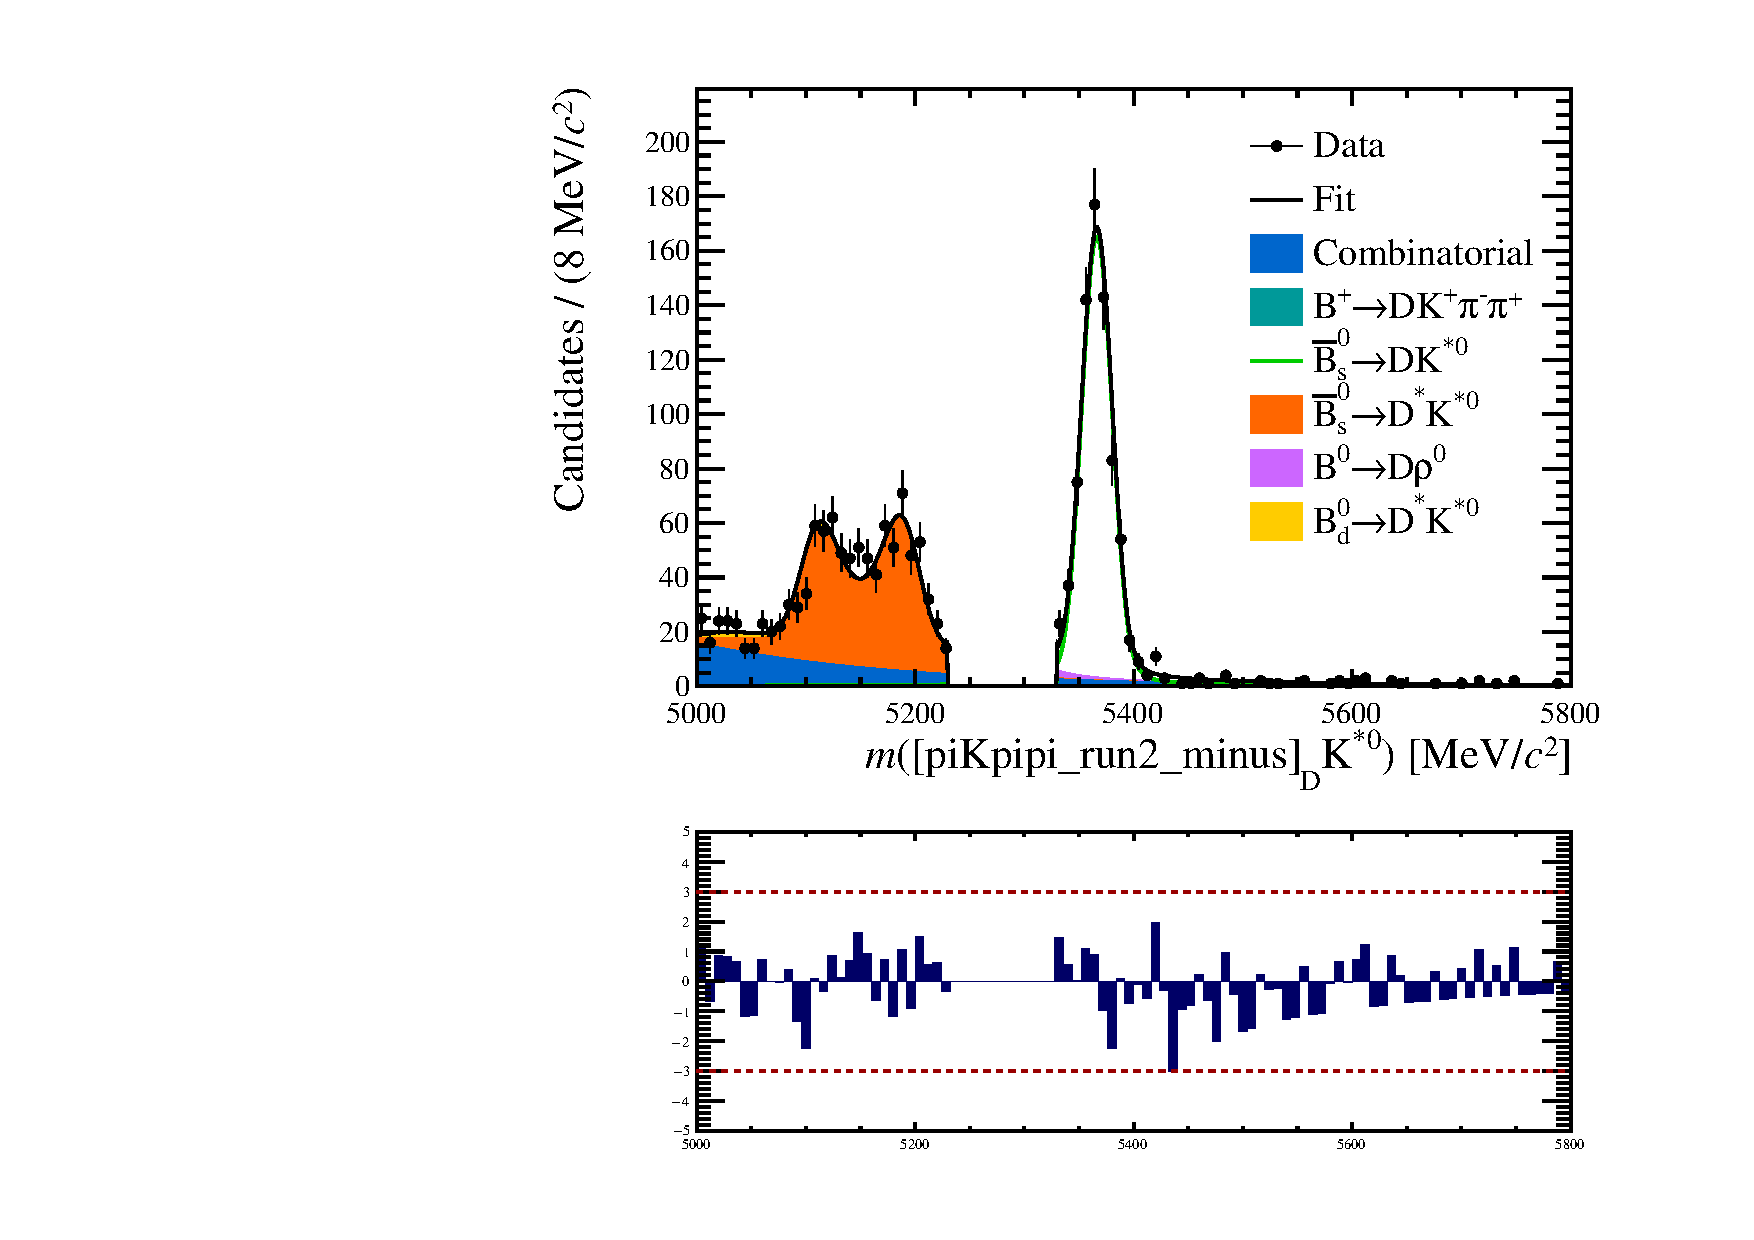
\includegraphics[width=0.45\textwidth]{ANA_resources/Plots/Data_fit/twoAndFourBody_data_split_piKpipi_run2_minus.pdf}} \\
    \end{tabular}
    \caption{Fit to $B$ invariant mass of selected candidates in the $\pi K\pi\pi$ final state, split by $B$ flavour and run.}
\label{fig:data_fit_piKpipi}
\end{figure}
\begin{figure}
    \centering
    \begin{tabular}{cc}
        \subfloat[][$B^0 \to D(\pi\pi\pi\pi)K^{*0}$ Run 2]{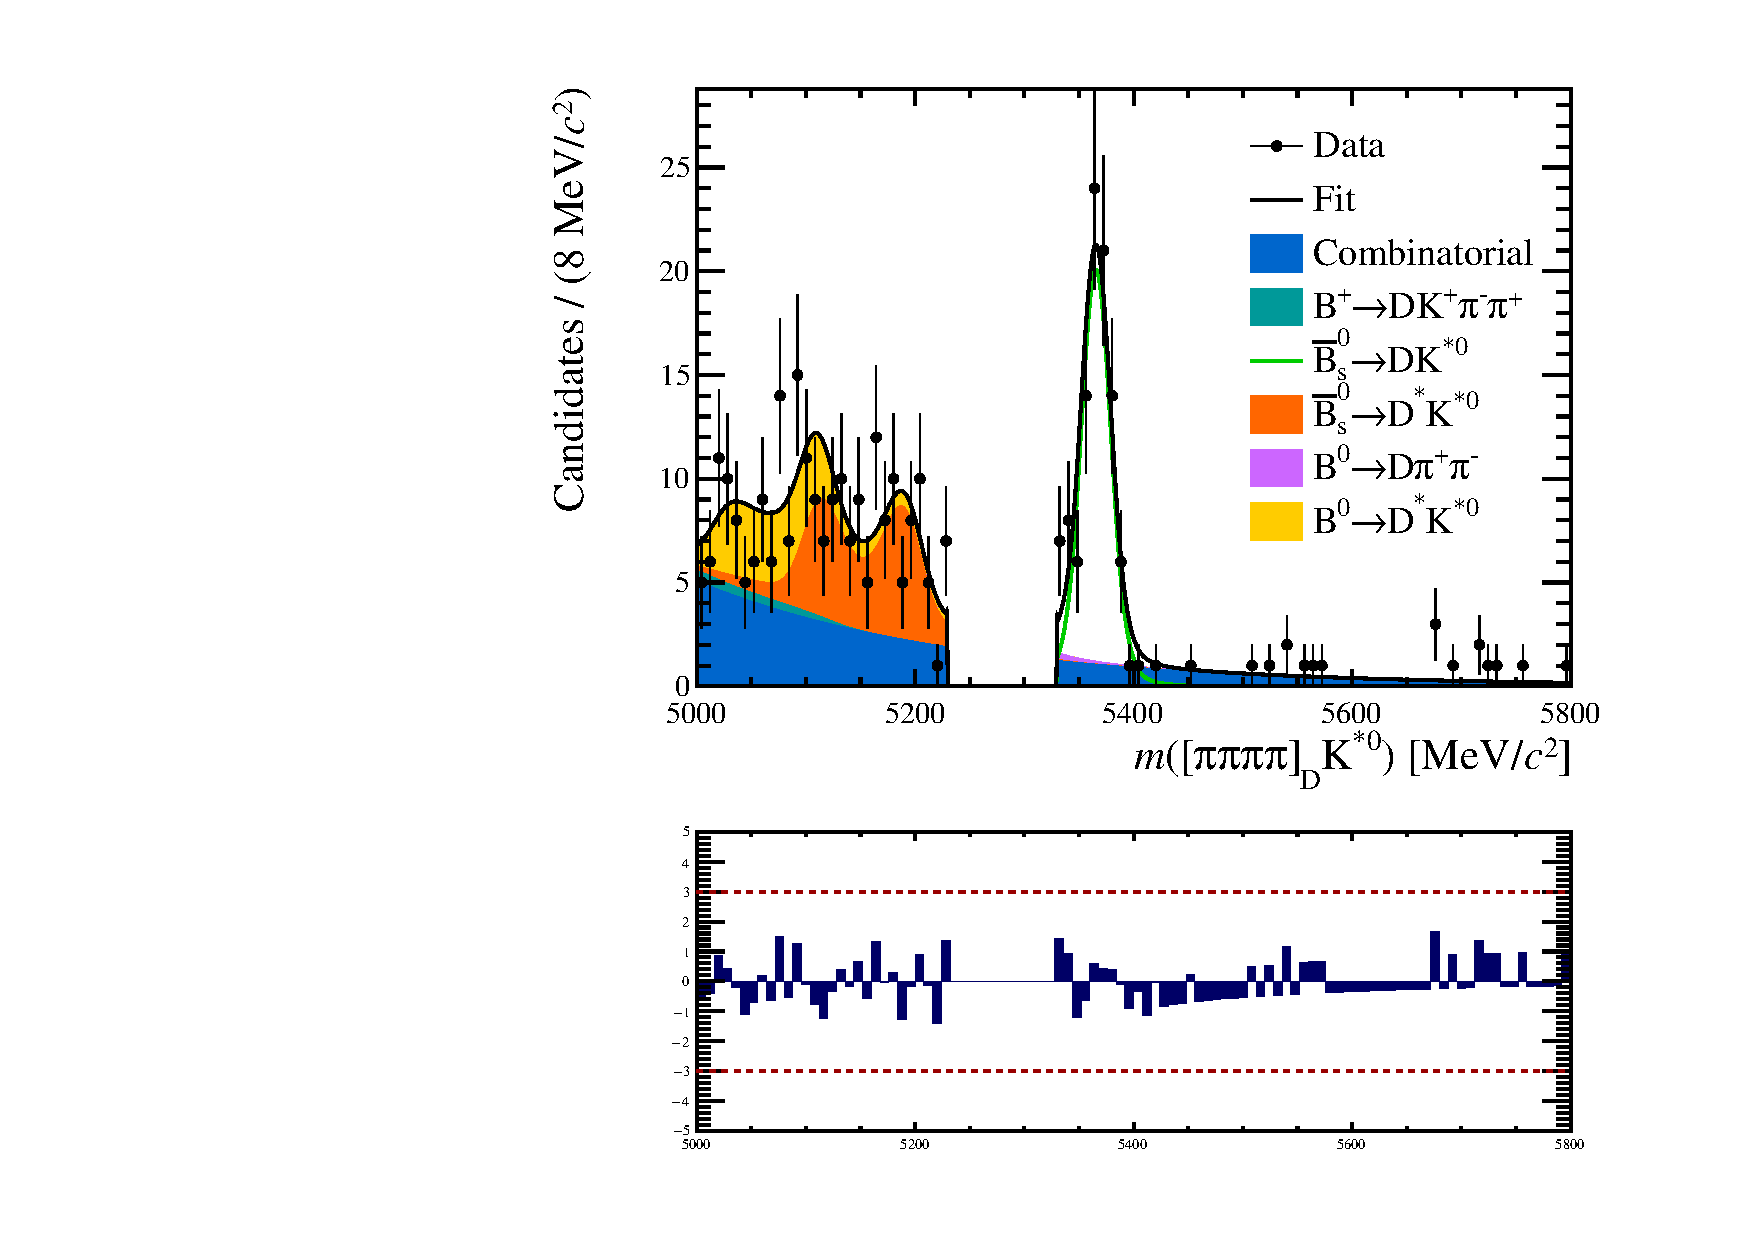
\includegraphics[width=0.45\textwidth]{ANA_resources/Plots/Data_fit/twoAndFourBody_data_split_pipipipi_run2_plus.pdf}} &
        \subfloat[][$\bar{B}^0 \to D(\pi\pi\pi\pi)\bar{K}^{*0}$ Run 2]{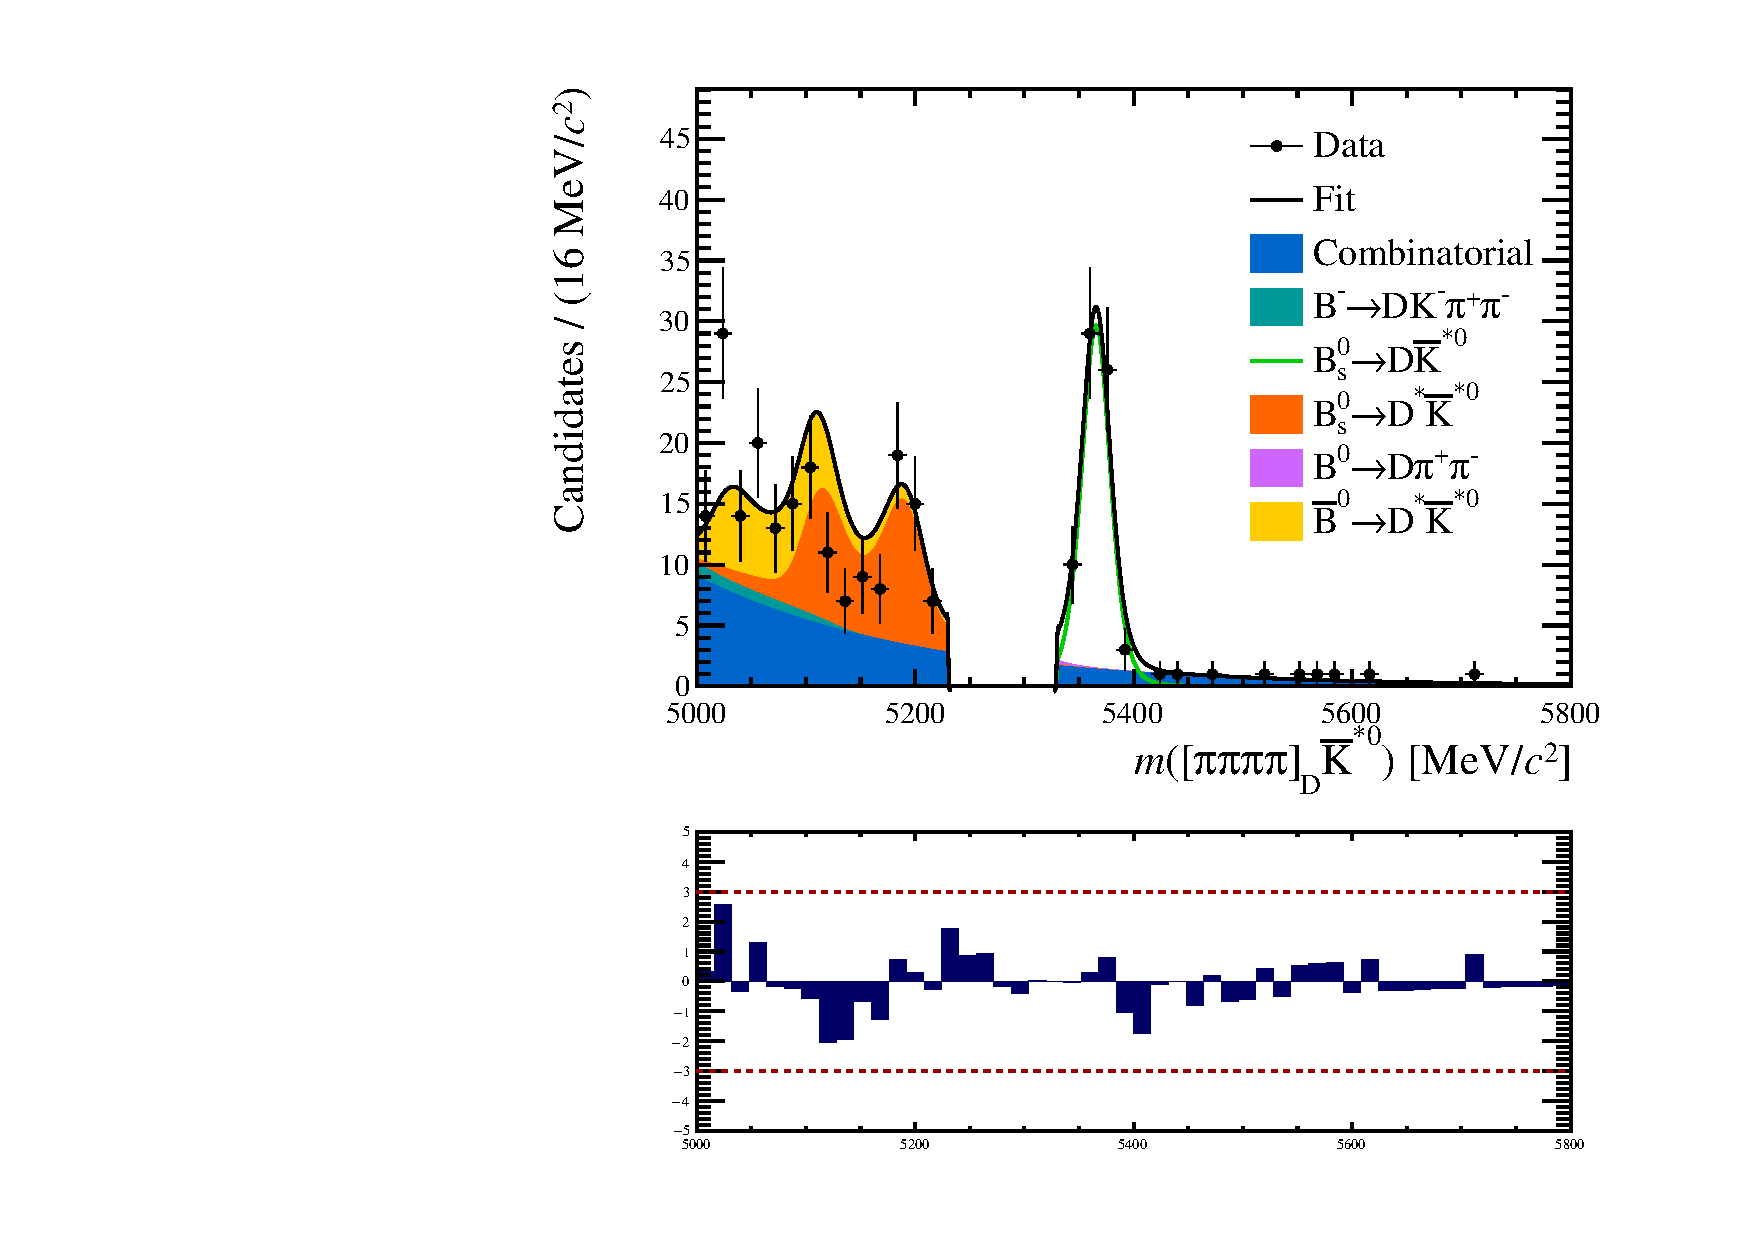
\includegraphics[width=0.45\textwidth]{ANA_resources/Plots/Data_fit/twoAndFourBody_data_split_pipipipi_run2_minus.pdf}} \\
    \end{tabular}
    \caption{Fit to $B$ invariant mass of selected candidates in the $\pi\pi\pi\pi$ final state, split by $B$ flavour and run.}
\label{fig:data_fit_pipipipi}
\end{figure}
